\chapter{Modelagem e Implementação}
    \section{Modelagem}
        
        %  entendemos o contexto do problema, levantamos requisitos, agora vamos modelar e tentar aplciar padro~eos de projeto pra facilitar
        
        Ao compreender o problema e suas limitações e especificidades, pode-se partir para modelar uma solução para tal.
        
        É uma prática comum no desenvolvimento de software aplicar padrões de projeto, mais conhecidos como \textit{Design Patterns}, ou basear-se em alguma estrutura pré-estabelecida como fundação do desenvolvimento.
        %todo cite design patterns 
        
        Dessa forma, optamos por usar um framework já bem consolidado: O Actor Framework, que é a implementação do modelo de atores em Labview. Isto será melhor descrito logo abaixo.
        
        Outro ponto importante desta etapa é saber representar o modelo desenvolvido. Em engenharia de software, a ferramenta mais utilizada neste processo é a Linguagem de Modelagem Unificada (do inglês \textit{Unified Modeling Language ou UML}, que nos permite representar o sistema de forma padronizada.
        
                
    \section{Um proposta do sistema dentro do modelo de atores}     
        A configuração de atores e responsabilidades propostas podem ser vistas na figura \ref{fig:modelo}. 
        
        Separamos em cinco classes de atores: comunicação serial; ator de multímetro; gerador de arquivo de registro de teste; Teste de powermeter; e controlador.
        \begin{figure}
            \centering
            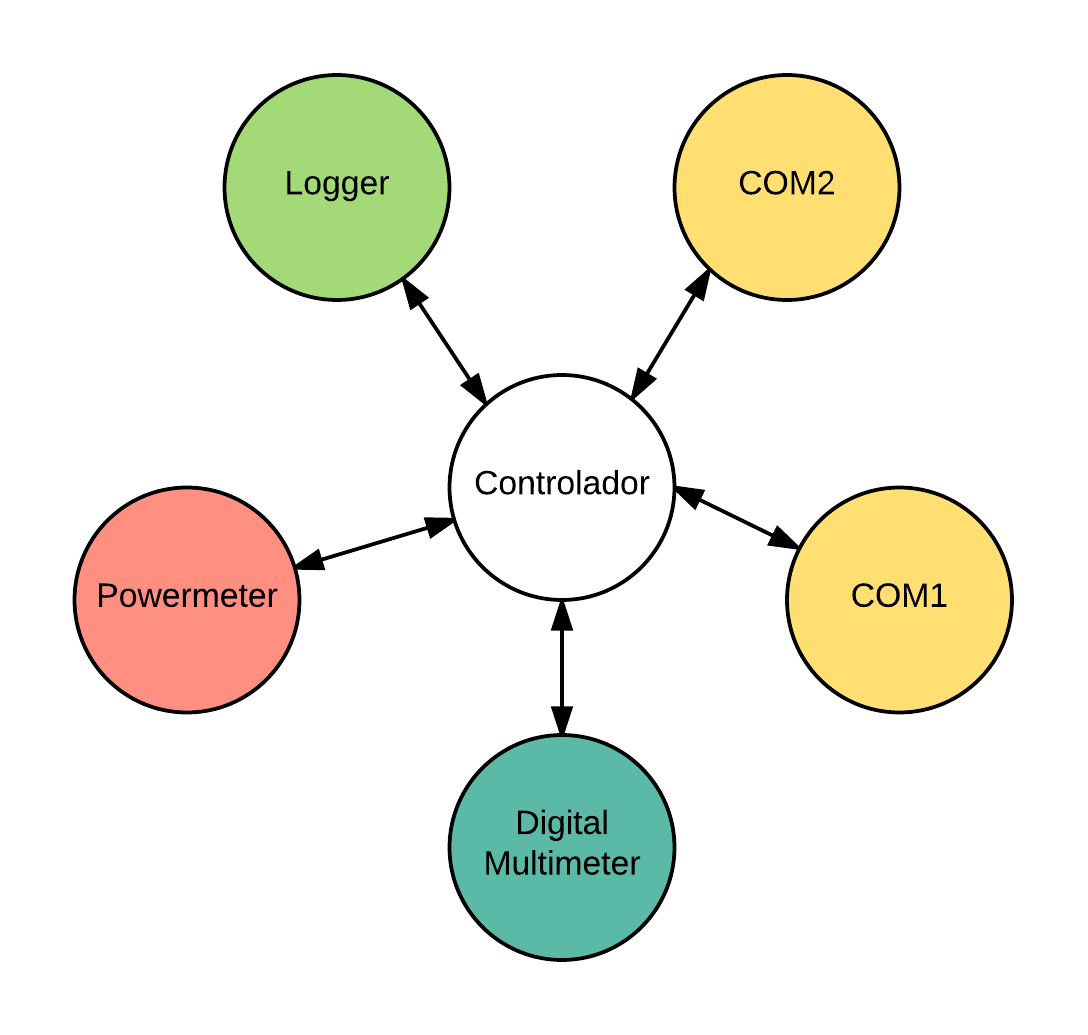
\includegraphics[width=0.9\linewidth]{fig/sistemmodel}
            \caption{Modelo do sistema no framework de atores}
            \label{fig:modelo}
        \end{figure}
            
        \subsection{Ator de comunicação serial}
            Ator responsável por enviar comandos de teste e verificar as respostas recebidas do dispositivo sob teste.
            
            Usamos dois atores no sistema pois trabalhamos com duas portas: uma para comunicar com o módulo por comandos AT, e outra para acessar periféricos conectados no barramento  I$^{2}$C. 
            
            Toda resposta aos comandos é verificada e relatada ao Ator Controlador, que por sua vez decide o fluxo de execução do roteiro de teste. 
            
            Devido ao curto prazo dado ao projeto, nessa implementação inicial não foi implementado o interpretador para o padrão de roteiros utilizados no programa anterior. o que daria bastante flexibilidade à equipe para editar o roteiro conforme mudanças de \textit{firmware}, aplicação ou revisões de placa. Ao invés disso, todos os comandos são parte do código fonte do programa, situação conhecida como \textit{hardcoding}. No contexto desse projeto isto é considerado um antipadrão de projeto de software, já que assumimos que variável ambiental é constante. %todo cite anti patterns
        \subsection{Ator Multímetro}
            \label{dmmmodel}
            
            Esta entidade é responsável pela leitura da porta RS232 do multímetro e transformar essas leituras em informações com mais sentido, e em uma interface de usuário ergonômica para o operador. Além disso, é interessante que o ator receba os vetores de teste para validar com as medidas.
            
            O multímetro utilizado é um ICEL MD-6400, com suporte de comunicação por uma porta serial RS232. A figura \ref{fig:dmmprotocol} exibe o funcionamento de seu protocolo, que a cada 250 ms, envia pacotes de 14 bits de dados a 9600 baudrate. 
            
            Logo, as primeiras etapas do algoritmo do multímetro seria ler e sincronizar os dados lidos pela porta serial. A sincronização é facil de implementar por meio de uma máquina de estados. Já a parte de decompor os dados do \textit{bitstream} em informação inteligível, vai desde a transformar números em código de sete segmentos em inteiros, a asssociar unidades de medida.
            
            Outra funcionalidade importante seria a de indicar o uso de um modo de operação incorreto, como por exemplo uso do instrumento como ohmímetro quando a medida era de tensão.
            
            Conforme mencionado no levantamento de requisitos do programa, são feitas quatro medições de tensão na placa. Os vetores de teste possuem os seguintes atribuitos: \textit{limiar máximo; limiar mínimo; unidade de medida; quantidade de novas tentativas permitidas}.
            
            Na sessão de implementação, será mencionado as melhorias na ergonomia do operador.
            
            \begin{figure}
                \centering
                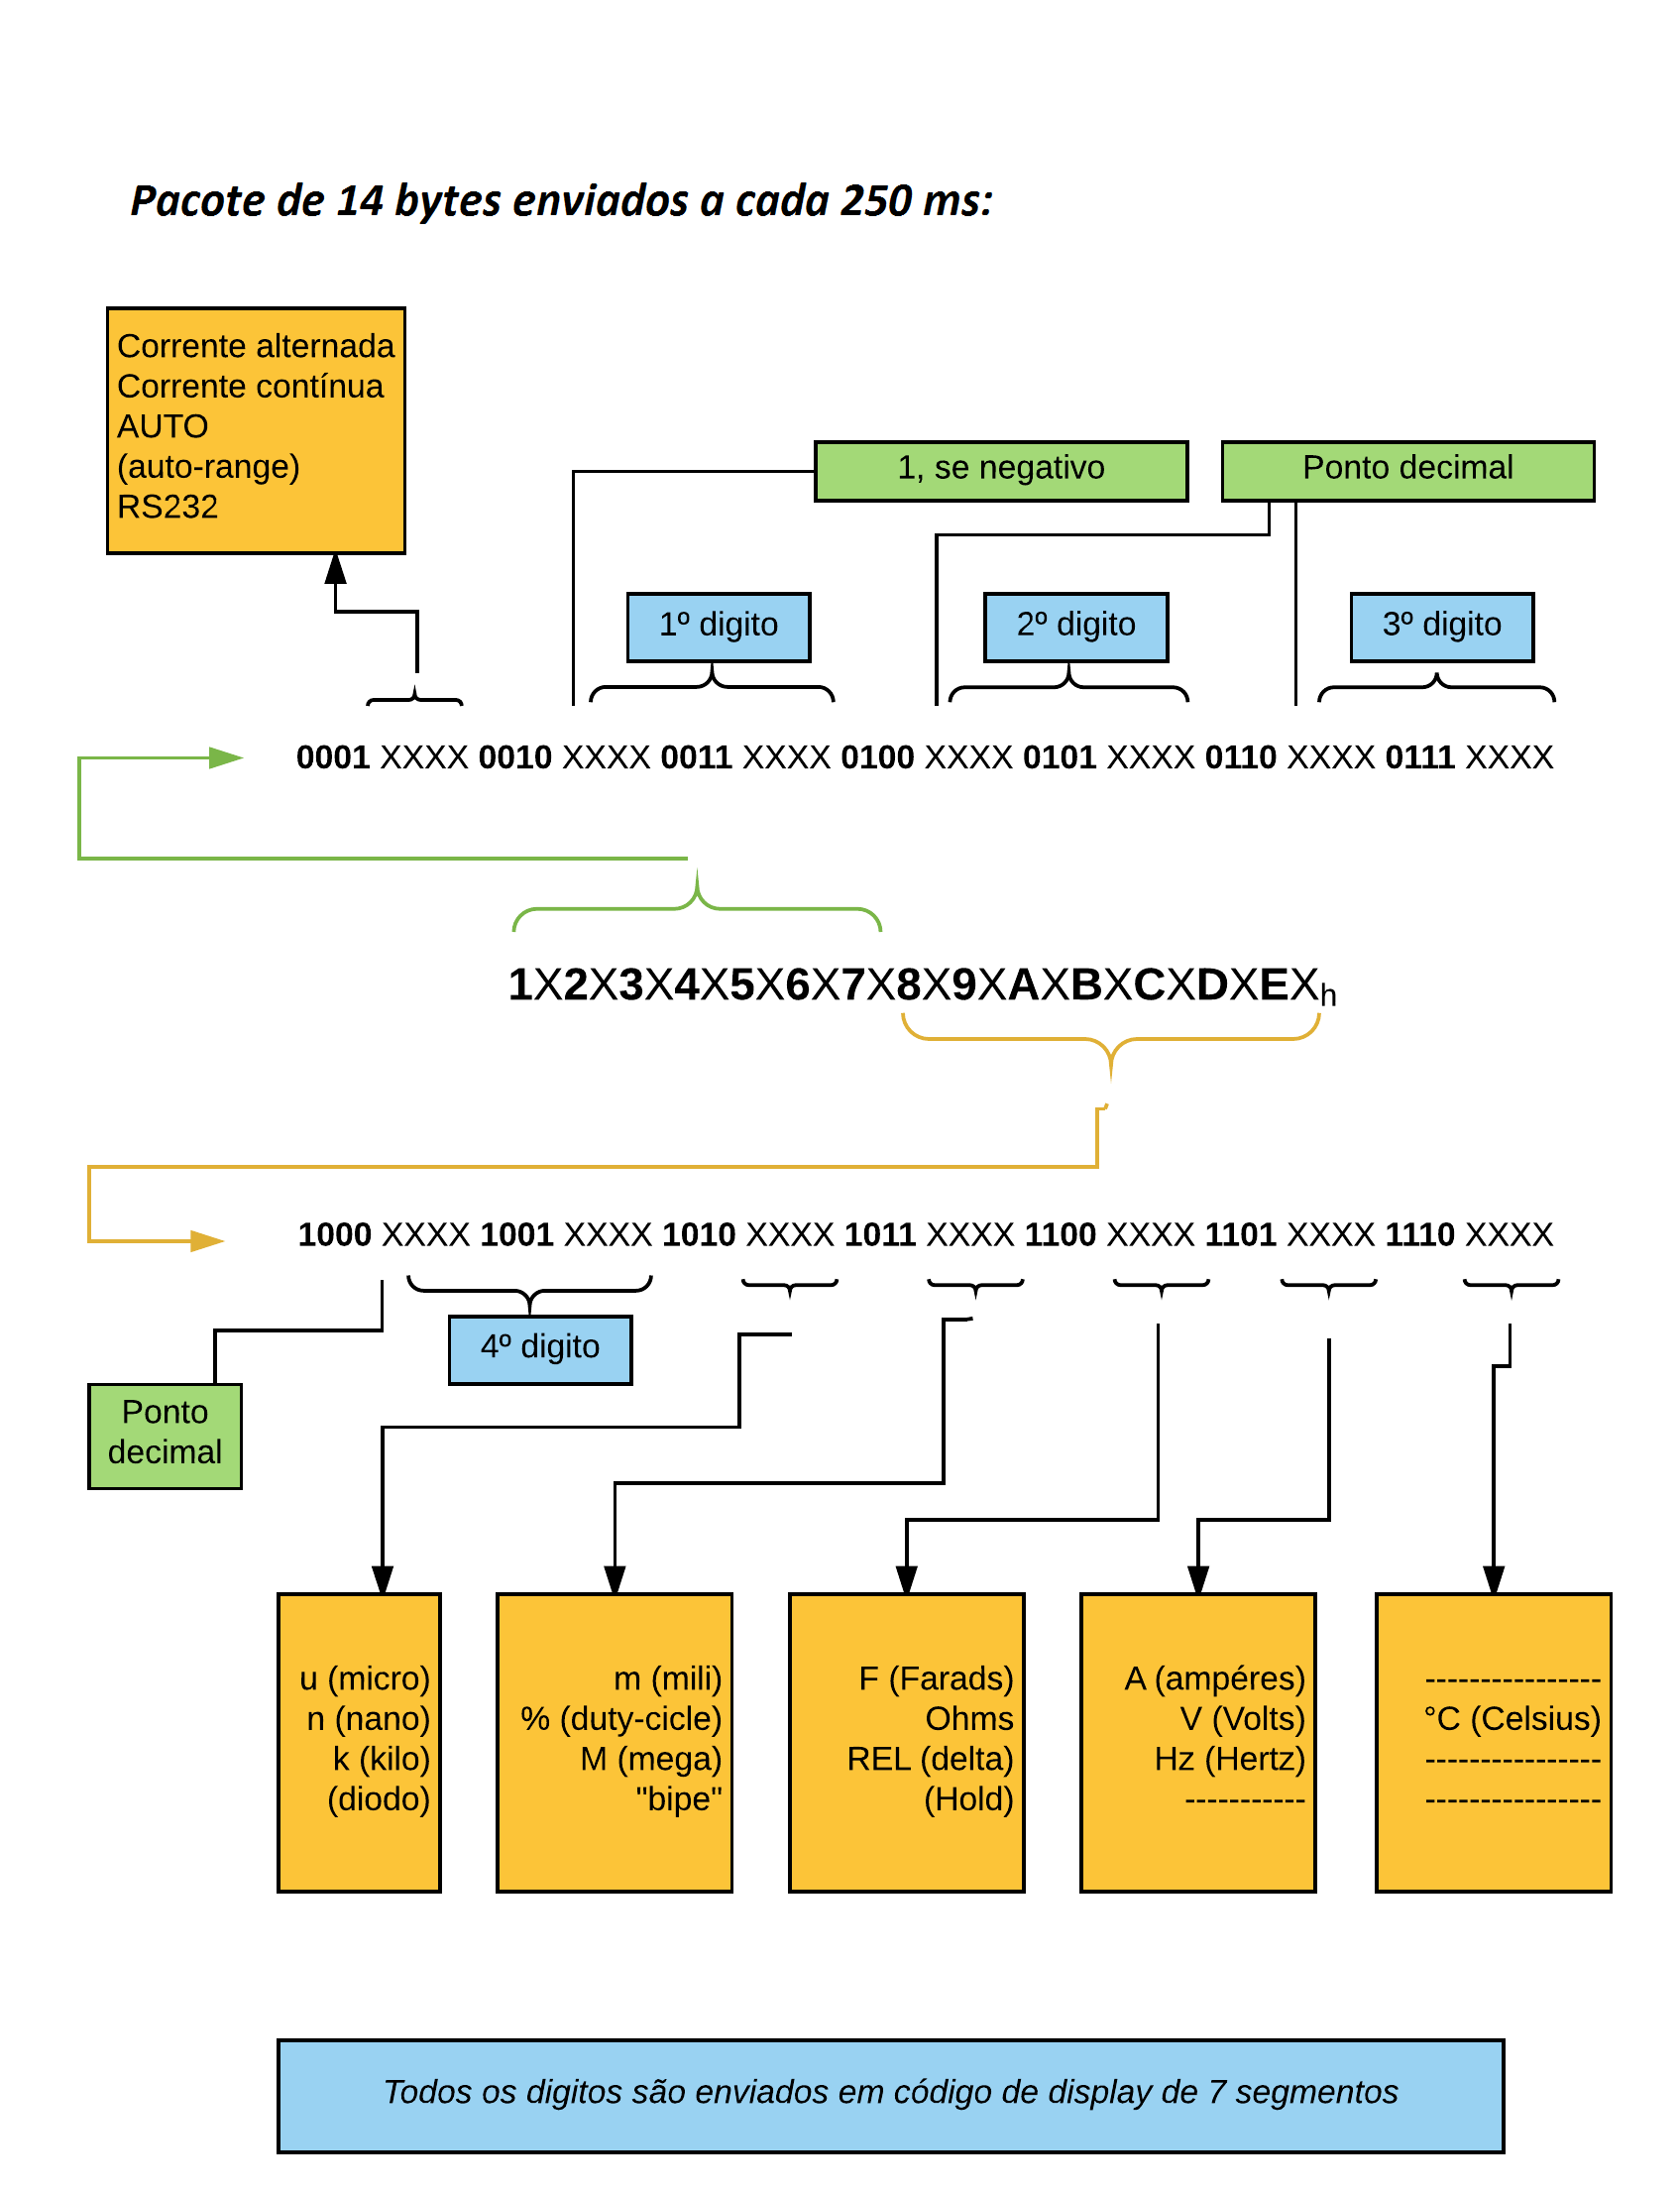
\includegraphics[width=\textwidth]{model/dmmprotocol}
                \caption{Protocolo de comunicação do multímetro}
                \label{fig:dmmprotocol}
            \end{figure}
            
        \subsection{Gerador de arquivos de registro}
        
            A saída principal do programa são os arquivos de registro, e para esta função foi designado um ator separado. 
            
            Dentre as suas funções estão: gerar um arquivo de registro completo do teste para fins de depuração e diagnóstico; gerar um arquivo de registro resumido só para o controle de qualidade em produção, e envio do registro para a base de dados dos produtos da empresa. E paralelo a isto foi desenvolvido um novo servidor de registros de teste com uma API própria.
            
            Este ator é alimentado pelo Controlador com informações do teste para preencher o arquivo de registro. 
            
        \subsection{Teste de potência do \textit{front-end}}
            \label{pwmodel}
        
            Ator que detém o controle do medidor de potência RF, também referenciado como \textit{Powermeter}. Este ator recebe como parâmetro a frequência de medição, o número de medidas, e os limites máximos e mínimos de de potência tolerados.
            
            O instrumento de medição de potência RF utilizado foi o NI 5680, da National Instruments, que mede potência RMS de sinais até 6 GHz, em larguras de banda bem estreitas (10-100 Hz de banda), e um alcance de potência de -40 dBm a +23 dBm.
            
            As baterias de testes estruturais e funcionais são quase todas realizadas dentro das empresas que realizam a montagem de placas, porém, o alto custo, a empresa possui só uma unidade deste instrumento, utilizado alternadamente entre o setor de manutenção e no final de produção. Por isso, a etapa de medição de potência de front-end é feita separada do demais testes e ainda não foi introduzida neste programa. 
            
            Para contornar isso foi feito um programa separado responsável por este teste, realizado no fim de linha de produção, antes de embalar o produto. E no programa deste trabalho, foi inserido a estrutura básica para implementação do medidor de potência de front-end.
            
        \subsection{Controlador}
            
            O controlador, como o próprio nome define, detém a responsabilidade sobre o fluxo de execução do programa, criando e destruindo os outros atores-módulos e fazendo a comunicação entre seus atores filhos. Além disso, detém a interface de usuário principal do programa. 
    
    \section{Modelagem UML}
        
        Para ilustrar o modelo do sistema estabelecido, foi escolhido representá-lo por um diagrama em linguagem universal de modelagem - UML, que é uma linguagem de uso geral dentro da engenharia de software, cuja a intenção é providenciar uma maneira padrão de representar o projeto de um sistema.
        
        \begin{comment}
        
        O padrão UML possui duas categorias de representação de software: Estrutural e Comportamental. Dentro dela temos:
        
            \begin{itemize}
                \item Diagramas Estruturais
                \begin{itemize}
                    \item Diagrama de Classes
                    \item Diagrama de Objetos
                    \item Diagrama de Componentes
                    \item Diagrama de Estrutura Composta
                    \item Diagrama de Instalação ou de Implementação
                    \item Diagrama de pacotes 
                    \item Diagrama de perfil
                \end{itemize}
                \item Diagramas Comportamentais
                \begin{itemize}
                    \item Diagrama de Casos de Uso
                    \item Diagrama de Transição de estados
                    \item Diagrama de Atividade
                    \item Diagrama de Objetos
                    \item Diagrama de Interação
                    \begin{itemize}
                        \item Diagrama de Sequência
                        \item Diagrama de Interatividade
                        \item Diagrama de Colaboração
                        \item Diagrama de Tempo ou Temporal
                    \end{itemize}
                \end{itemize}
            \end{itemize}
        
            Jà foi descrito o funcionamento nuclear de um ator Por sua simplicidade e também pelo seu compo estar descrito em seus ara representar este sistema, a representação será restrita aos diagramas de classe, e transição de estados.
            
            \subsection{Diagrama de estados}
            \subsection{Diagrama de sequências}
        \end{comment}
        
        \subsection{Diagrama de classes}
            %todo escrever alguma coisa
            \begin{figure}
                \centering
                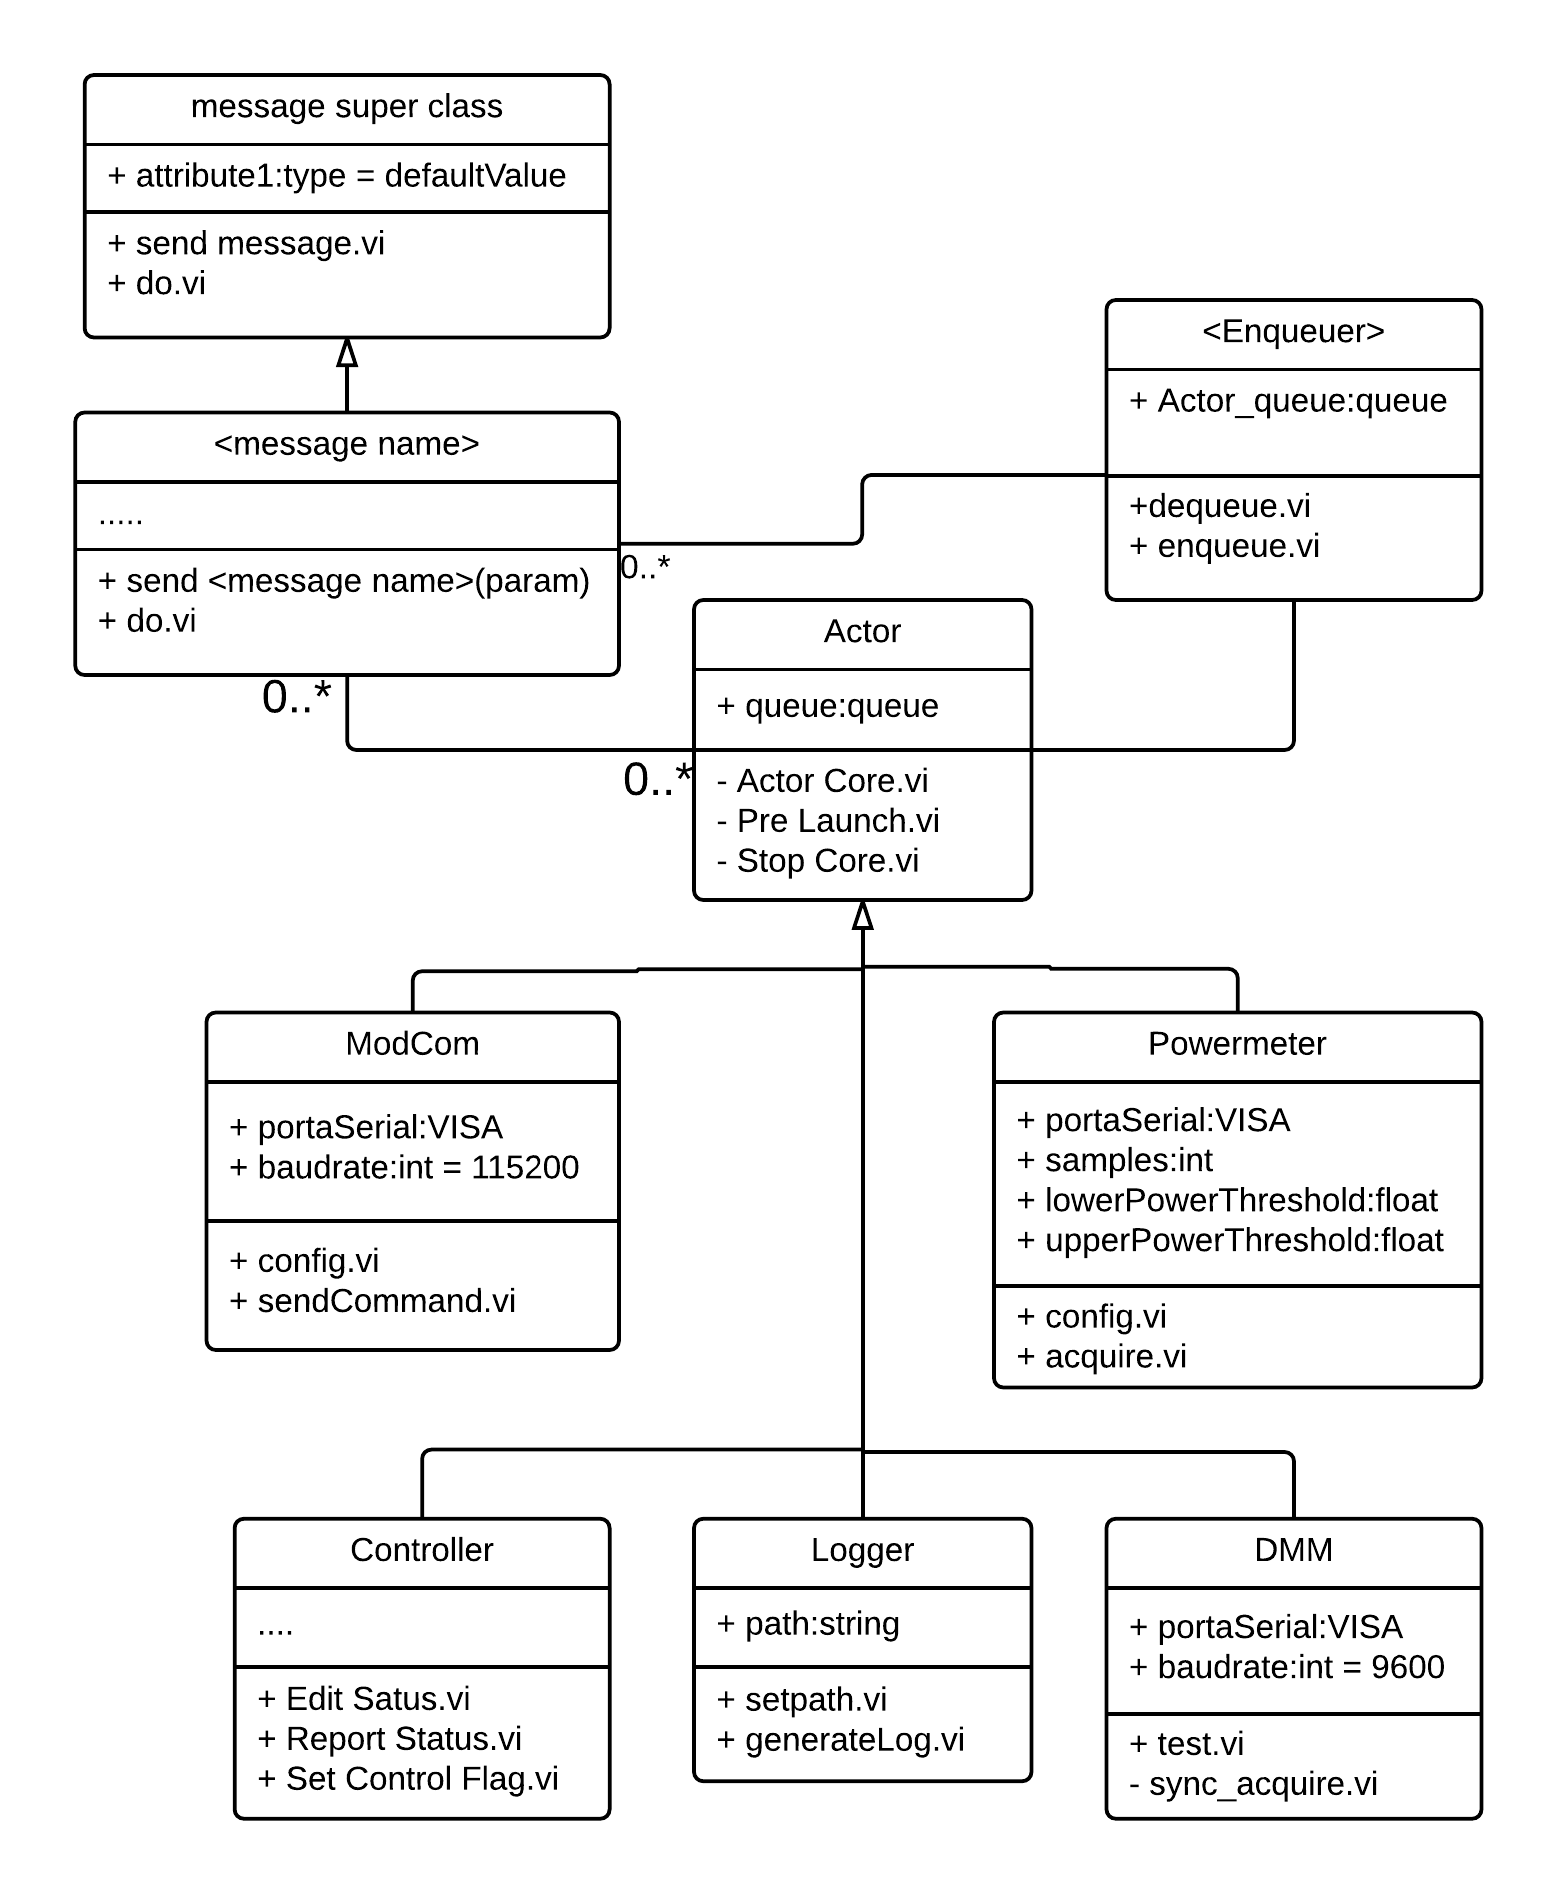
\includegraphics[width=1.4\linewidth, angle=90]{model/class}
                \caption{Diagrama de classes}
                \label{fig:classdiagram}
            \end{figure}
            
            %https://decibel.ni.com/content/docs/DOC-42227
        
        \subsection{Fluxograma da bateria de testes}
            O Fluxograma da bateria de testes é exposto na figura \ref{fig:flowchart}. Este é o fluxograma do roteiro de testes que se mantém desde antes do início deste trabalho. Nota-se que a única etapa fracionada para execução concorrente é o teste das bandejas de cartões SIM. 
            
            Por simplificação esta estrutura foi inicialmente mantida, mas trabalhos futuros serão realizados para a otimização do roteiro.
            
            \begin{figure}
                \centering
                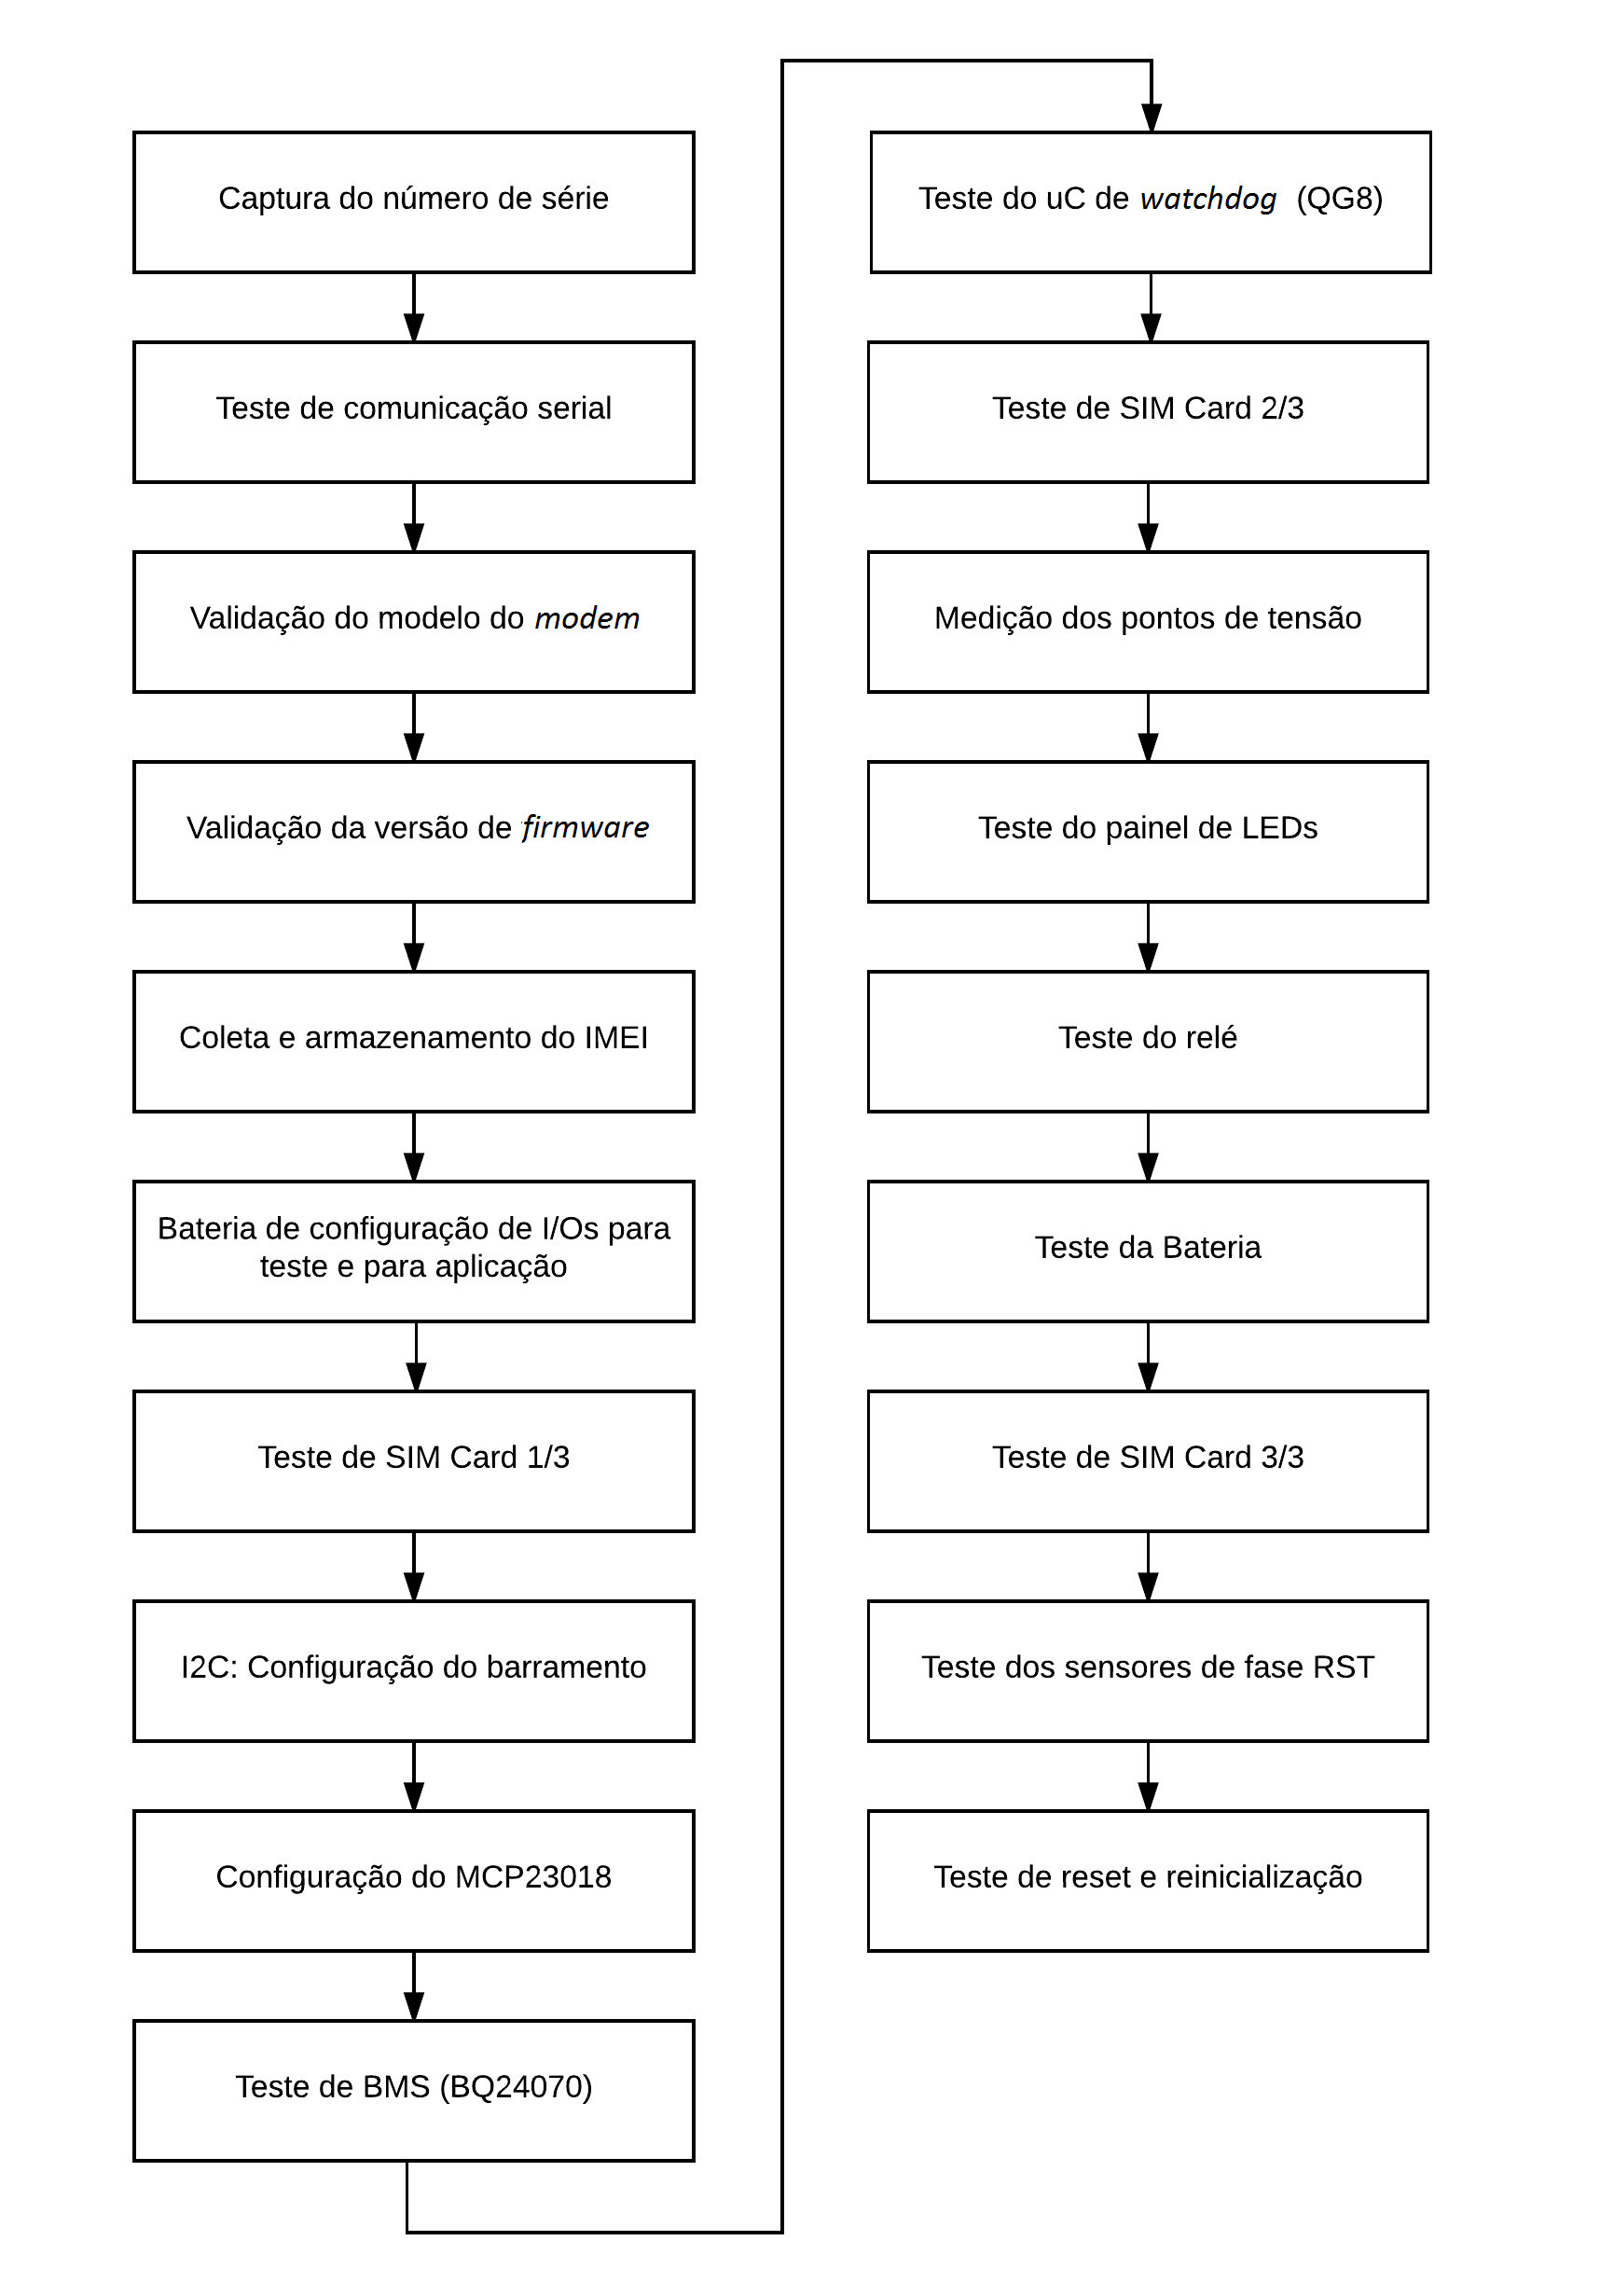
\includegraphics[width=\textwidth]{model/fluxograma}
                \caption{Fluxograma da bateria de testes}
                \label{fig:flowchart}
            \end{figure}
        
    \clearpage
    \section{Implementação}
    
        A ultima sessão foi dedicada a entender e modelar o problema a partir de uma solução proposta. Nesta sessão descreveremos a implementação dos módulos do programa de teste sob a perspectiva do modelo de atores e do framework de atores da Labview.
        
        Revendo a figura \ref{fig:modelo} vemos que o sistema em operação é composto por cinco módulos:
        \begin{itemize}
            \item Controlador;
            \item Módulo de Comunicação - \textit{Modcom};
            \item Gerador de Registros - \textit{Logger};
            \item Multímetro digital - DMM;
            \item Medidor de potência do \textit{front-end} - \textit{Powermeter}.
        \end{itemize} 
        
        Todos estes módulos possuem a implementação do \textit{framework}, através da herança da classe \textit{actor} e da classe \textit{actor message}. Todo ator tem que implementar a função \textit{actor core.vi} para poder alterar o comportamento do ator. Como o próprio nome diz, esta é a função núcleo do ator, e é responsável por inicializá-lo e executar o \textit{loop} de tratamento de mensagens. Também é possível, e recomendável, inserir nesta função, outras subrotinas, como, por exemplo, tratadores de eventos - que é um componente do controlador, que veremos a seguir.
        
        \subsection{Implementação do comunicador serial}
        
        A comunicação serial é feita por portas VISA (Virtual Instrument Software Achitecture), que são o padrão da National Instruments para configuração, programação, comunicação, e solução de problemas de sistemas de instrumentação. No ambiente Labview, comunicações seriais são abertas por meio de uma camada VISA.
        
        Na figura \ref{fig:serialcored}, pode-se ver a função básica criada para realizar toda a comunicação com o modem da placa. Sua função é enviar comandos e esperar pela resposta padrão ou esgotamento do tempo de resposta.
        
        O diagrama de blocos do ator comunicador é mais enxuto do que o controlador, pois não possui uma estrutura reativa a eventos (figura \ref{fig:modcomcore}).
        
        Após sua configuração - porta serial a ser usada, \textit{baudrate}, etc - o ator está pronto para comunicar com o módulo. Após receber do controlador o bloco de testes para ser executado, o ator executa a rotina e reporta ao Controlador os dados de resposta, assim como o diagnóstico de aprovação ou reprovação.
        
        Um exemplo interessante de um dos blocos de teste pode ser visto na figura \ref{fig:modcomledd}. Este é o bloco de teste do painel LEDs do módulo, que permite que o usuário compare o painel do módulo físico à um \textit{pop-up} que emula como o painel deveria estar (figura \ref{fig:modcomledp}). Comparada à solução anterior, que era baseada em texto e com inserção de respostas via terminal, essa foi uma alternativa mais ergonômica para o operador, reduzindo erros e aumentando a velocidade desta etapa de teste.
            
        
        \begin{figure}
                \centering
                 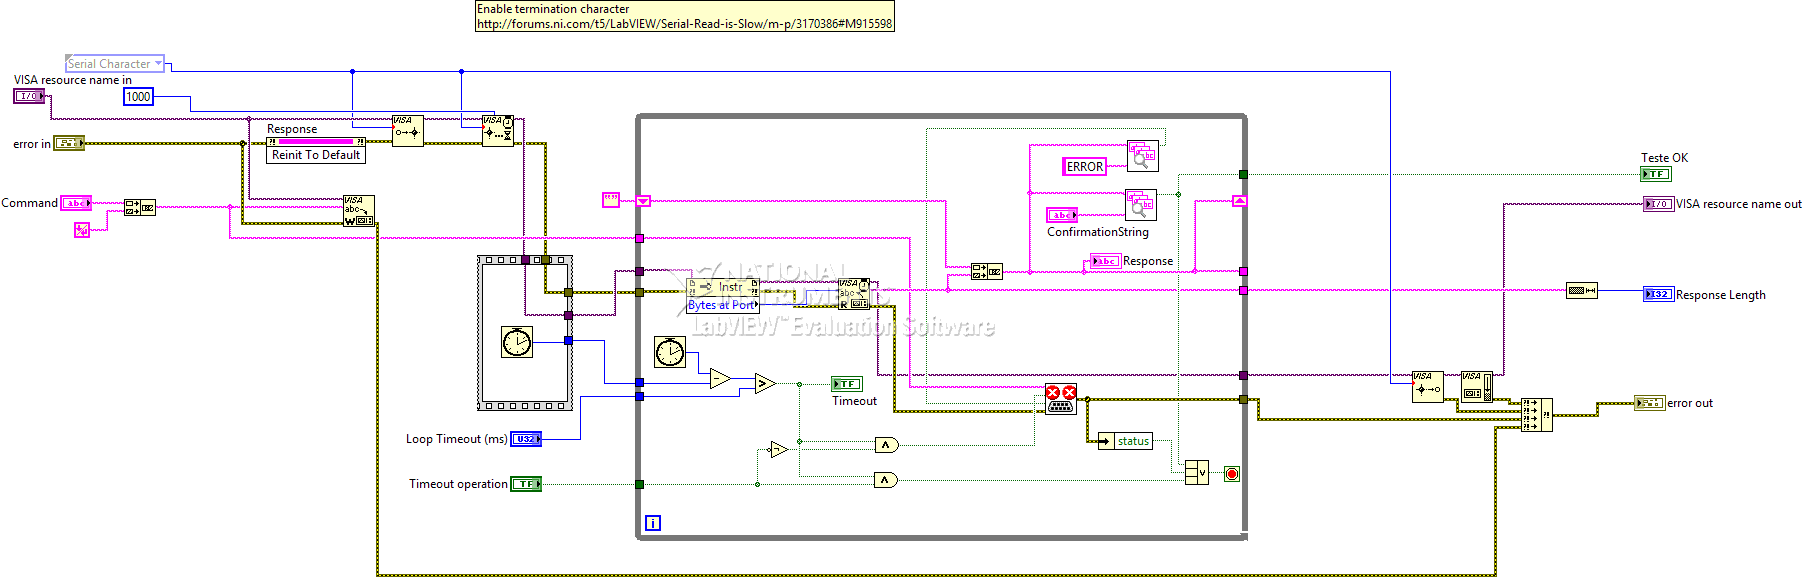
\includegraphics[width=1\linewidth]{lv/modcom/ModCOM_serialcored}
                \caption{Captura de tela da função básica de teste serial}
                \label{fig:serialcored}
        \end{figure}
        
        \begin{figure}
                \centering
                 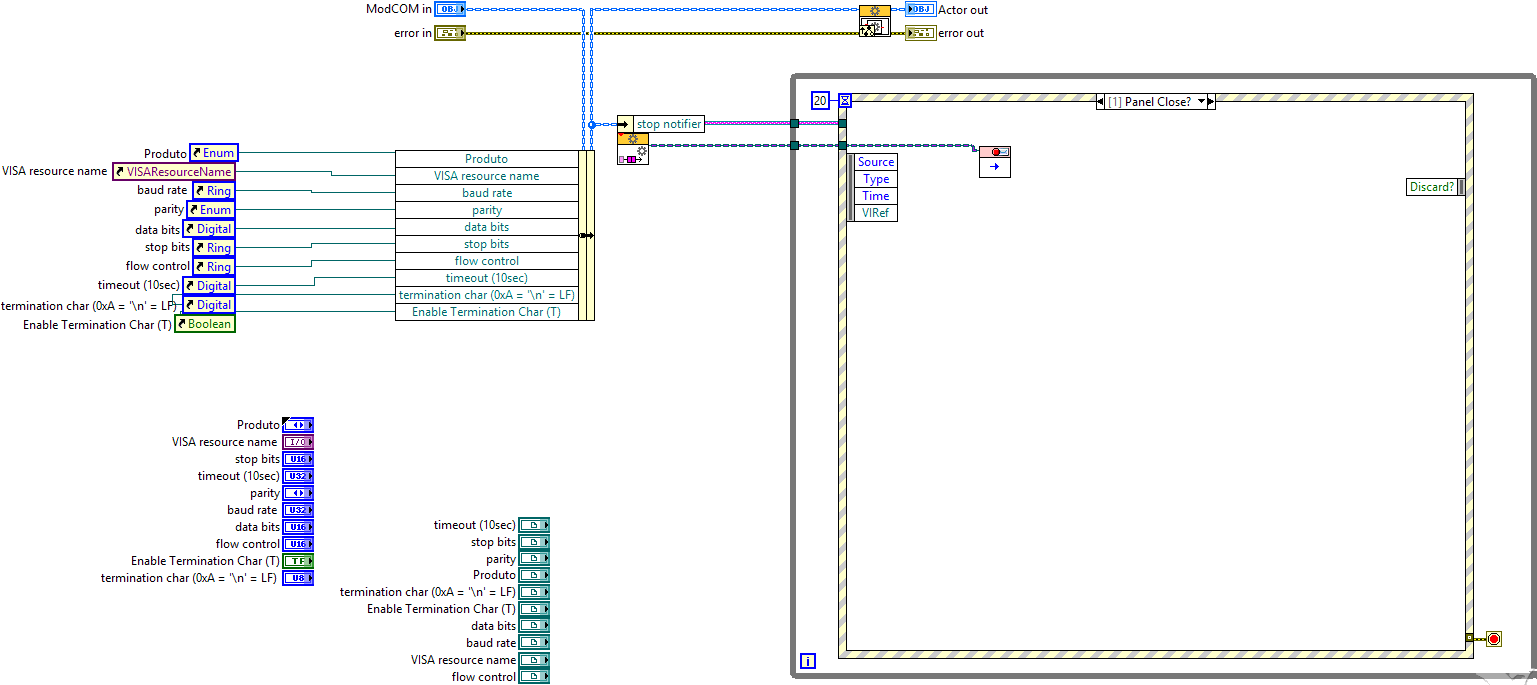
\includegraphics[width=1\linewidth]{lv/modcom/ModCOM_lvclass_Actor_Cored}
                \caption{Captura de tela do Actor Core do comunicador serial}
                \label{fig:modcomcore}
        \end{figure}
        
        \begin{figure}
                \centering
                 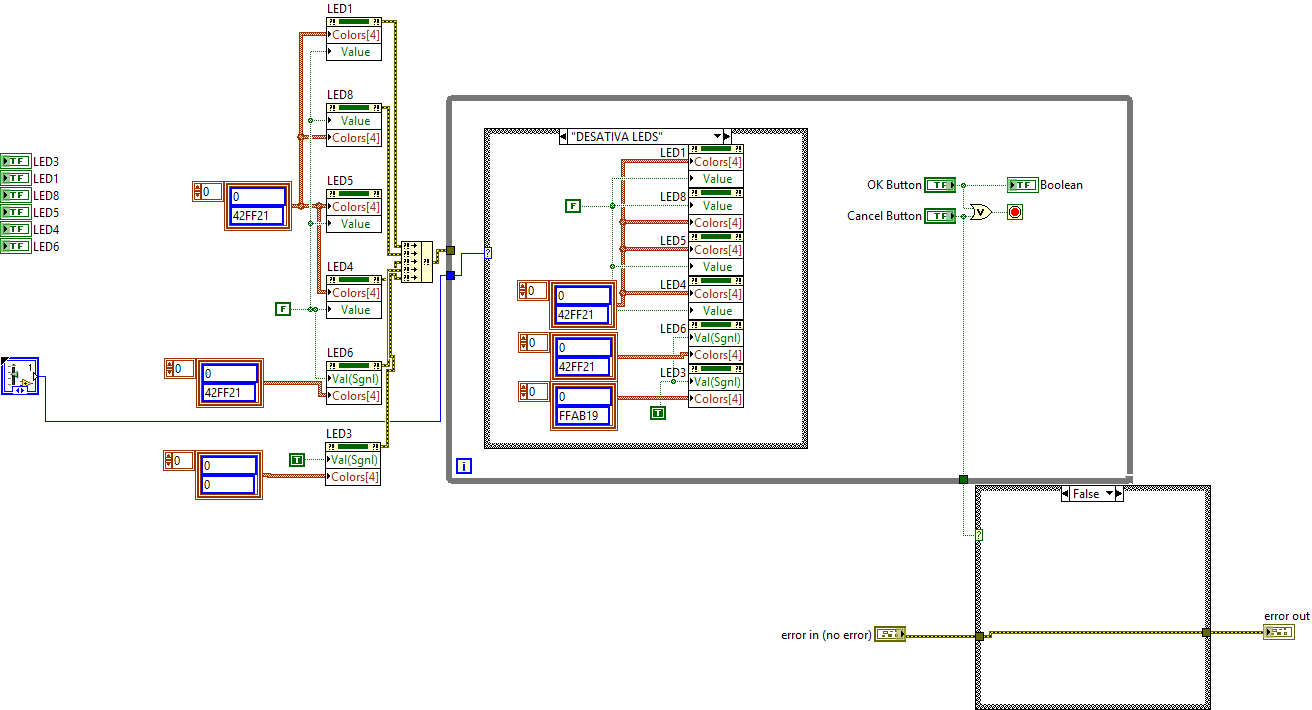
\includegraphics[width=1\linewidth]{lv/modcom/ModCOM_LED_popupd}
                \caption{Captura de tela do Diagrama de Blocos da rotina de testes de LEDs e GPIOs}
                \label{fig:modcomledd}
        \end{figure}
        
        
        
        \begin{figure}
                \centering
                 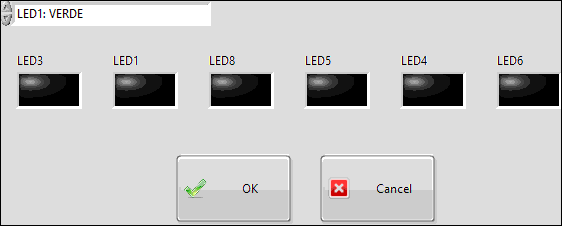
\includegraphics[width=1\linewidth]{lv/modcom/ModCOM_LED_popupp}
                \caption{Captura de tela do Painel Frontal de testes de LEDs e GPIOs}
                \label{fig:modcomledp}
        \end{figure}
        % parte oculta de diagramas
        \begin{comment}
        
         \begin{figure}
                \centering
                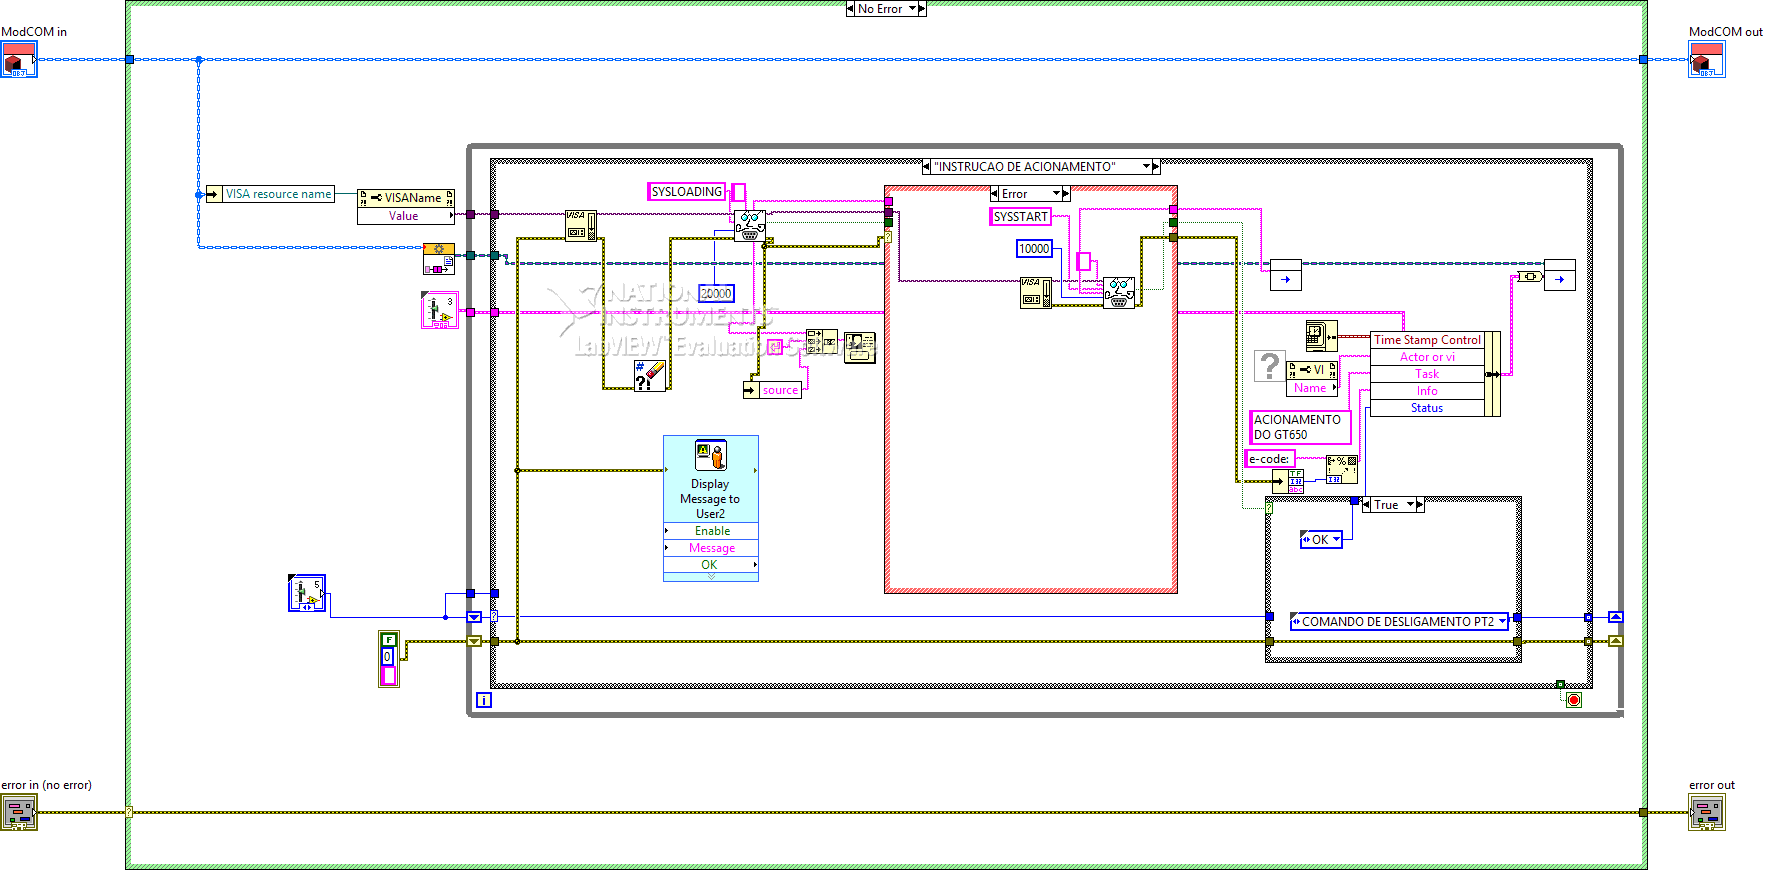
\includegraphics[width=1\linewidth]{lv/modcom/ModCOM_lvclass_desligamentoresetd}
                \caption{Captura de tela do Rotina de desligamento e reset do modem}
                \label{fig:modcomshutdown}
        \end{figure}
        
        
        \begin{figure}
                \centering
                 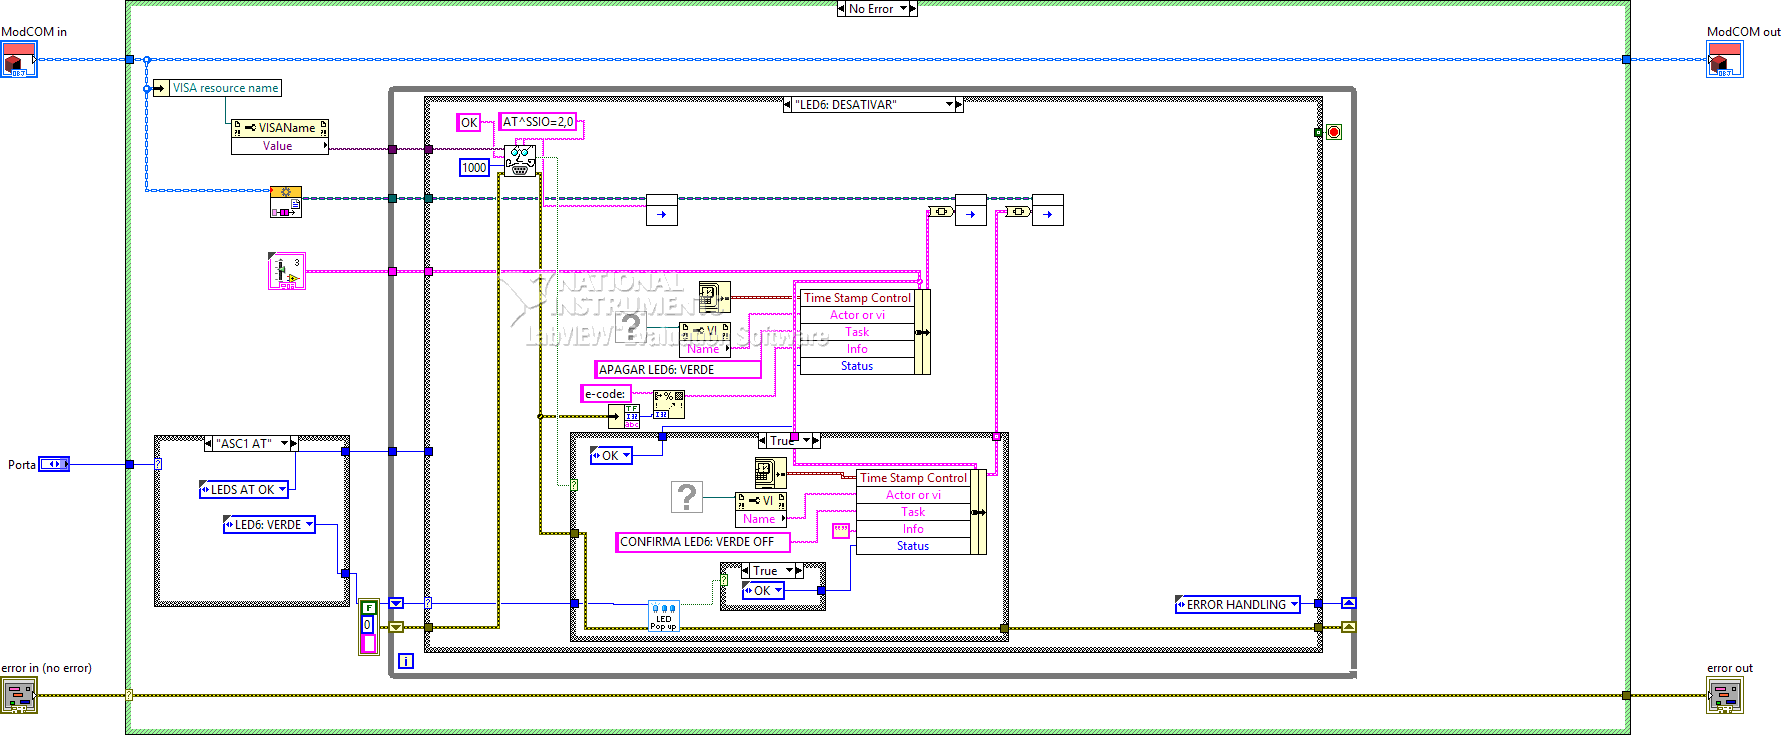
\includegraphics[width=1\linewidth]{lv/modcom/ModCOM_LED_I2Cd}
                \caption{Captura de tela do comunicador i2c}
                \label{fig:modcomledi2c}
        \end{figure}
        
        
        \begin{figure}
                \centering
                 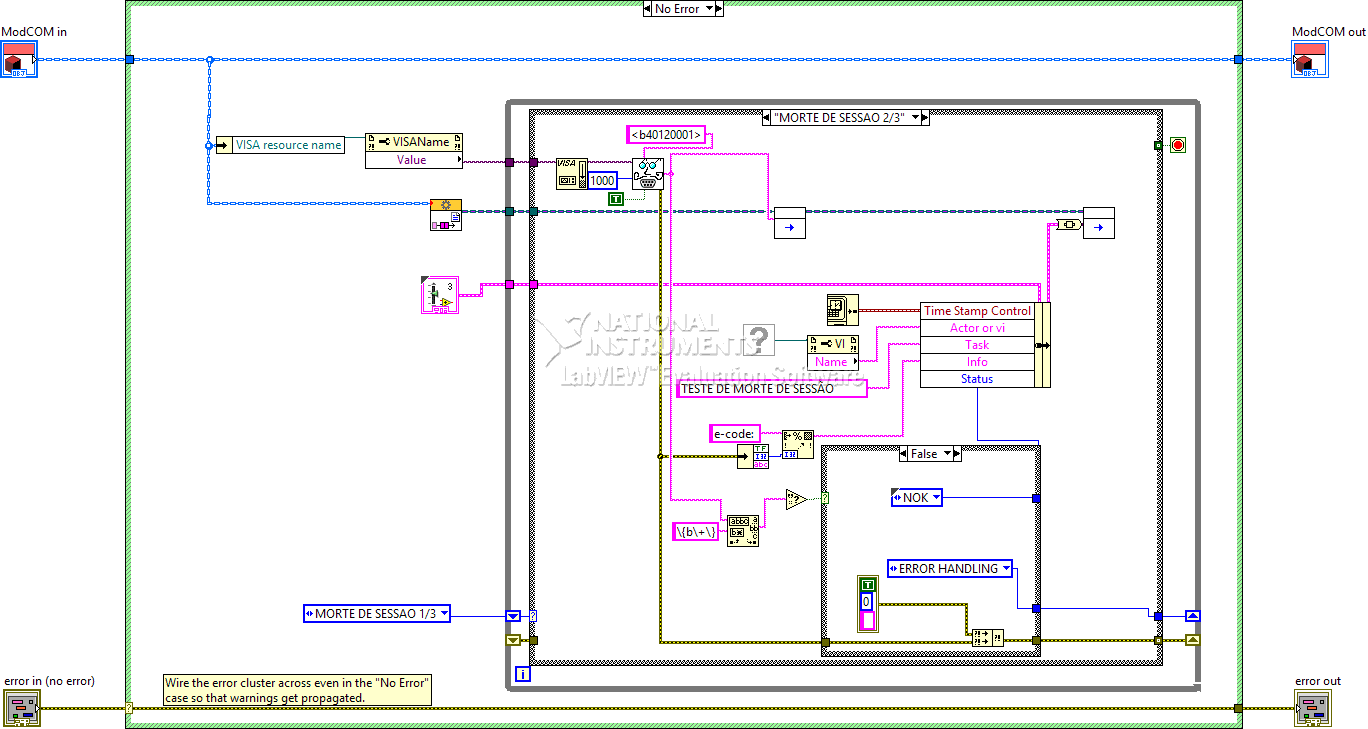
\includegraphics[width=1\linewidth]{lv/modcom/ModCOM_morted}
                \caption{Captura de tela do Teste de fechamento ou morte de comunicação serial}
                \label{fig:modcommorte}
        \end{figure}
        
        \begin{figure}
                \centering
                 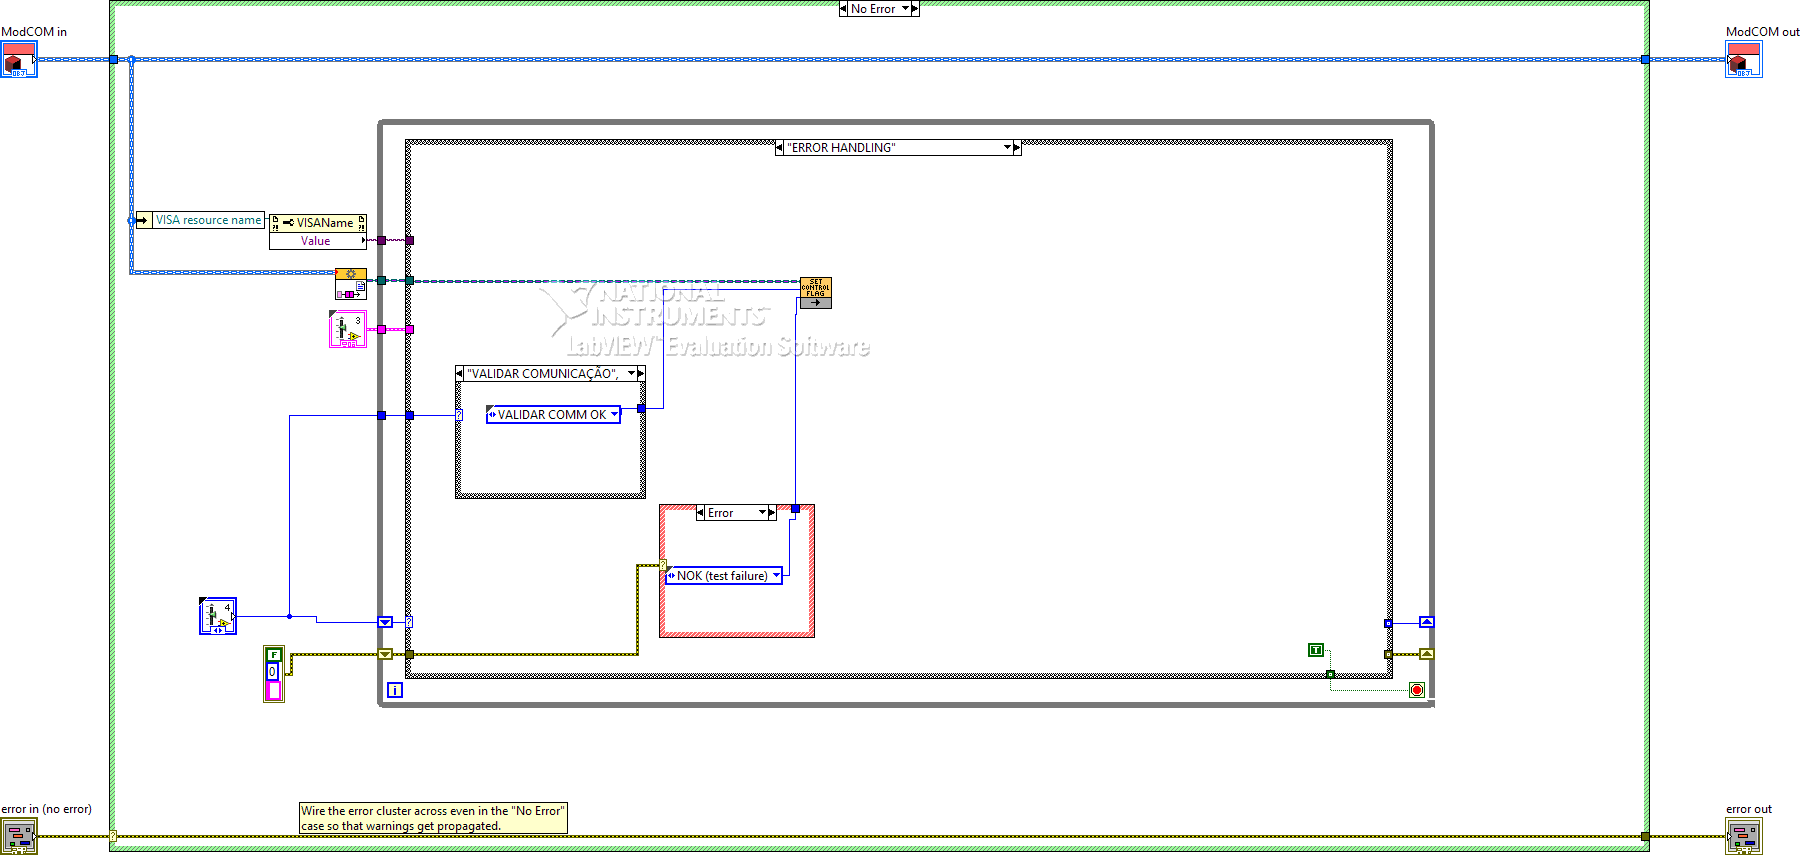
\includegraphics[width=1\linewidth]{lv/modcom/ModCOM_nopsutestd}
                \caption{Captura de tela do Captura de tela da rotina de teste sem fonte de alimentação}
                \label{fig:modcomnopsu}
        \end{figure}
        
        \begin{figure}
                \centering
                 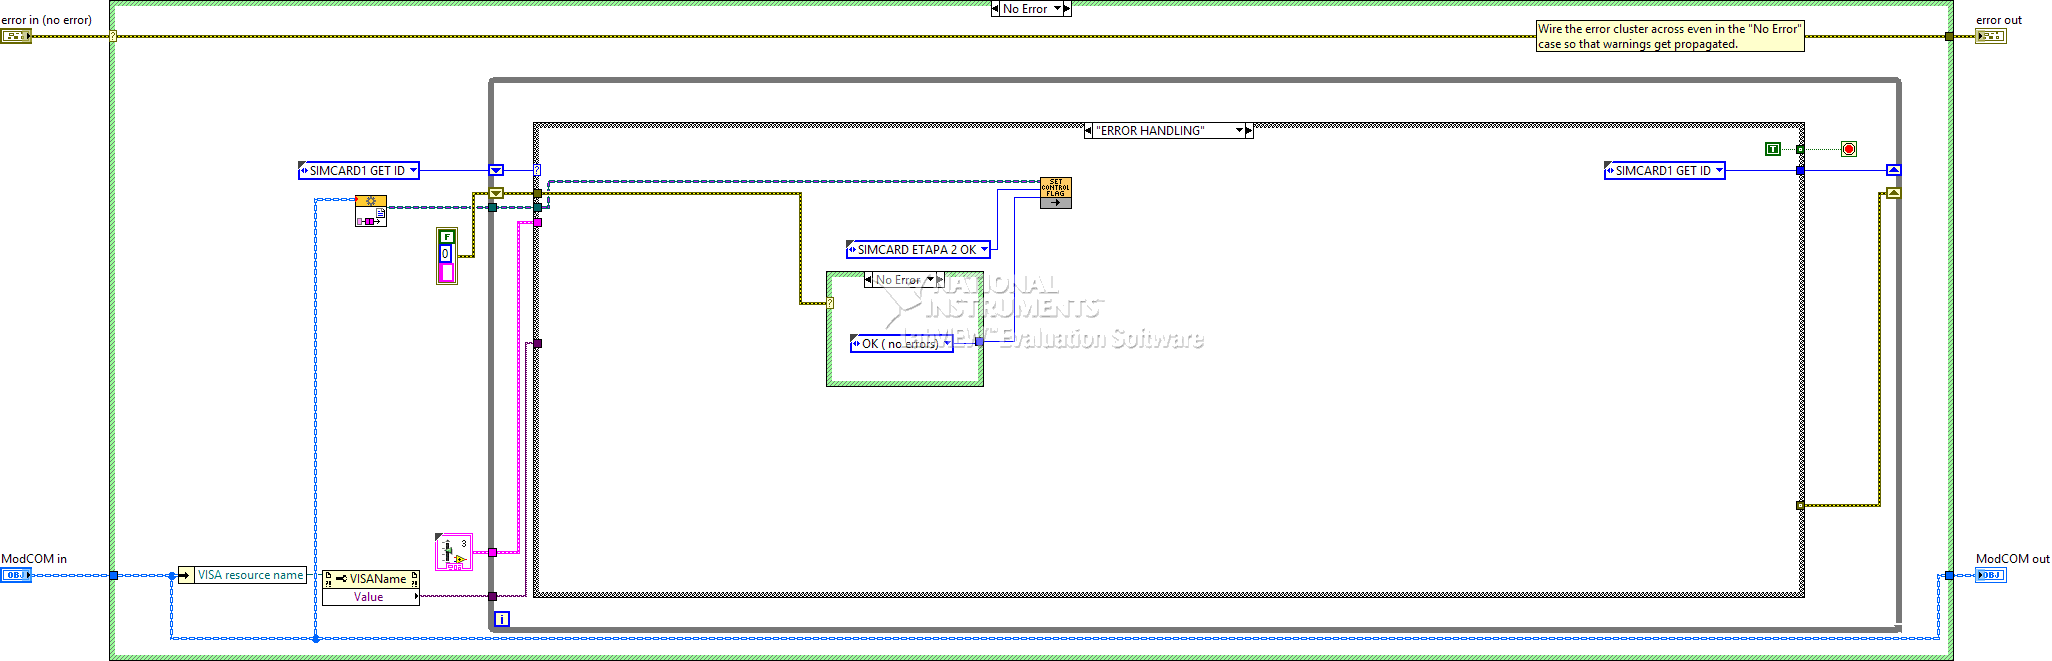
\includegraphics[width=1\linewidth]{lv/modcom/ModCOM_simcard}
                \caption{Captura de tela da rotina de teste dos simcard}
                \label{fig:modcomsimcard}
        \end{figure}
        
        \begin{figure}
                \centering
                 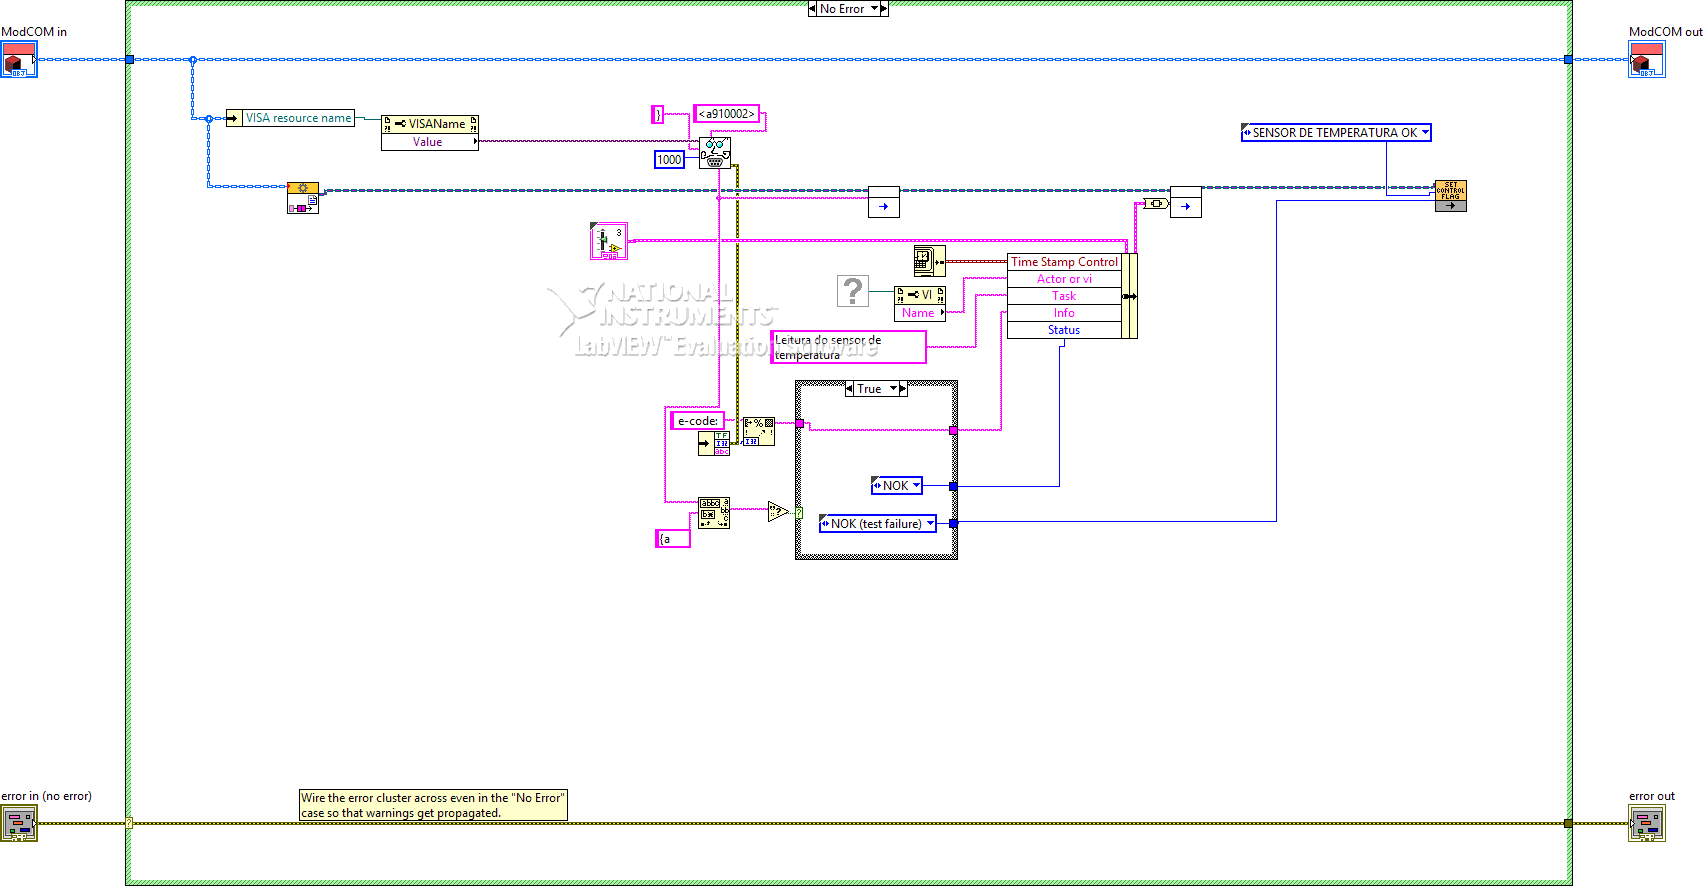
\includegraphics[width=1\linewidth]{lv/modcom/ModCOM_temp}
                \caption{Captura de tela da rotina de teste do sensor de temperatura}
                \label{fig:modcomtemp}
        \end{figure}
        
        
        \begin{figure}
                \centering
                 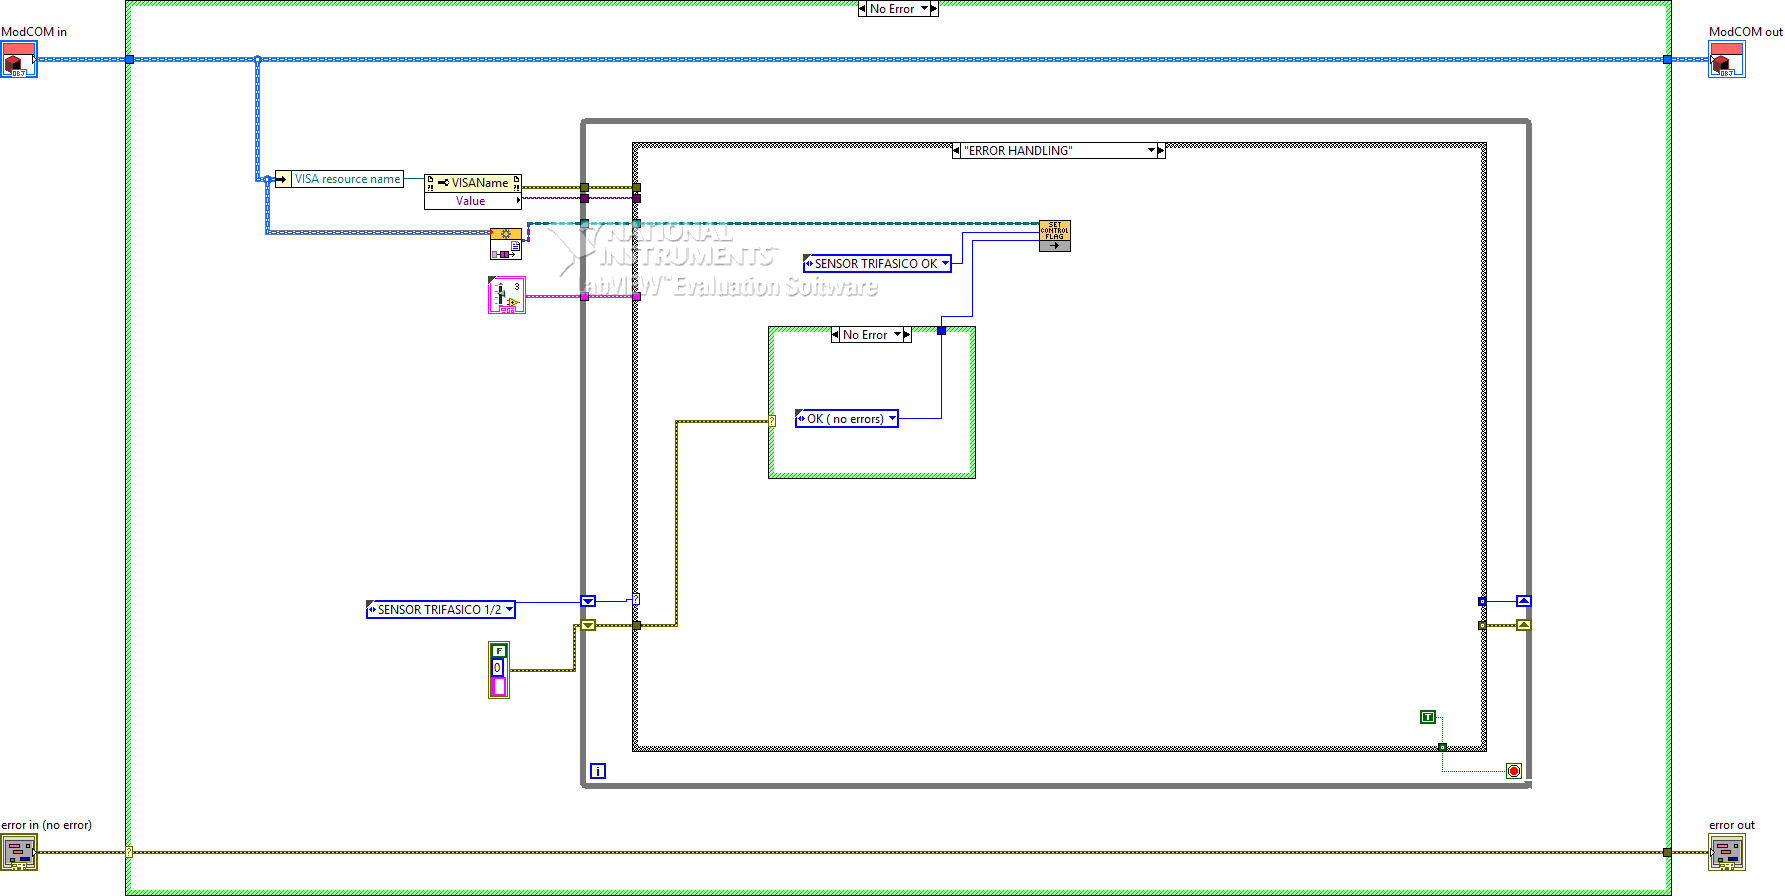
\includegraphics[width=1\linewidth]{lv/modcom/ModCOM_tritestd}
                \caption{Captura de tela da rotina de teste do sensor de presença das tensões trifásicas}
                \label{fig:modcomtri}
        \end{figure}
        
        \end{comment}
        
        \clearpage
        \subsection{Implentação do multímetro}
            % implementação Sincronização, máquina de estados 
            % figura com máquina de estados da leitura do multimetro
            %figura com os blocos e documentaçaõ da vi
            
            % vaiprecisar: diagrama de funcionamento do multimetro
            % na sessão anterior, um diagrama sobre o protocolo
            % aqui um diagrama de como lemos esse protocolo e fazemos parse
            
            Como mencionado na sessão de modelagem \ref{dmmmodel}, o ator responsável pelo multímetro precisa ler o \textit{bitstream} de leituras enviados pelo multimetro, e comparar e validar com os vetores de teste desejados.
            
            A implementação foi da seguinte forma: o \textit{bitstream} passa por uma etapa inicial de sincronização (figura \ref{fig:dmmacq}), até que se chegue ao inicio do pacote, em seguida entra em modo de aquisição, aonde o pacote é analisado e recebe significado (figuras \ref{fig:dmmbitcode} e \ref{fig:dmmparser}). Com a informação pronta, os dados vão para a interface de usuário, e junto com os vetores de pontos de teste informados pelo controlador, os valores lidos são validados em um algoritmo similar a um \textit{debouncer} (figura \ref{fig:dmmfpbd}). Explicando melhor: \textit{Se as leituras do multímetro permanecerem dentro dos limites tolerados para um determinado ponto de teste durante um período de 1 segundo, a medição é aprovada.} 
            
            Voltando à questão ergonômica, o operador não precisa tirar sua atenção da ponta de prova nos pontos de teste para ter que digitar respostas no terminal do programa. O \textit{debouncer} automaticamente passa para os próximos pontos de teste à medida que o ponto de teste é validado. E além das referencias da Interface Gráfica de Usuário (figura \ref{fig:dmmfp}), o programa emite indicações sonoras específicas em caso de aprovação, reprovação, ou nova tentativa.
            
            \begin{comment}
            \begin{figure}
                \centering
                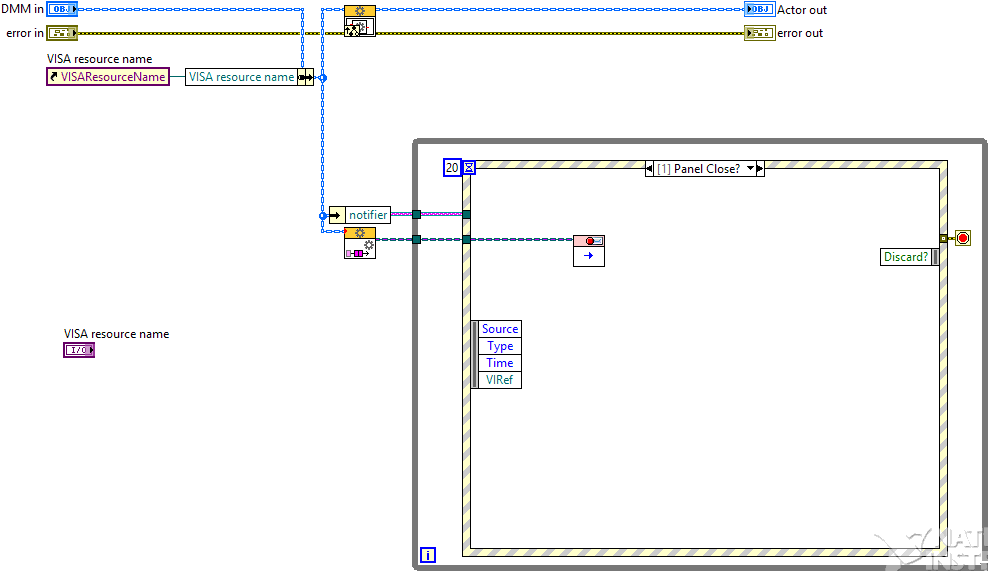
\includegraphics[width=1\linewidth]{lv/dmm/DMM_lvclass_Actor_Cored}
                \caption{Captura de tela do Actor Core do Multimetro}
                \label{fig:dmmcore}
            \end{figure}
            
            \end{comment}
            \begin{figure}
                \centering
                 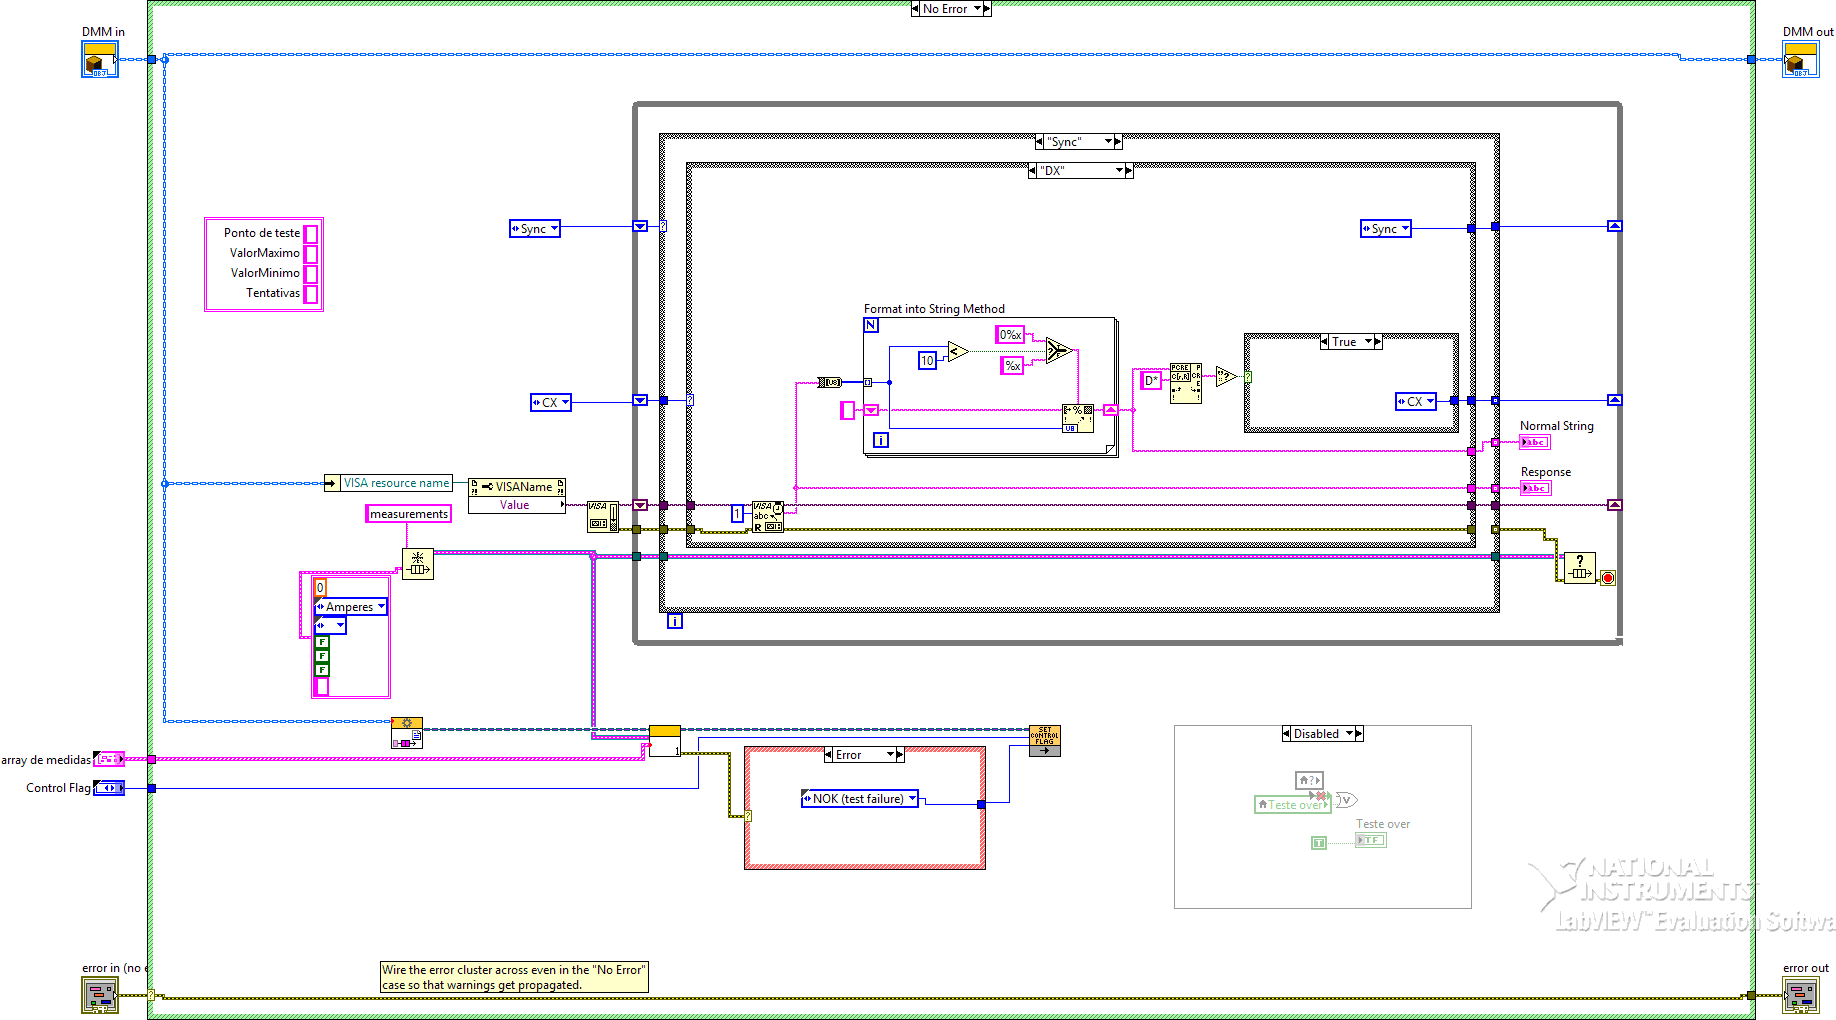
\includegraphics[width=1\linewidth]{lv/dmm/DMM_lvclass_AcquireTestpointsd}
                \caption{Captura de tela do Aquisição de dados pela serial}
                \label{fig:dmmacq}
            \end{figure}
            
            
            \begin{figure}
                \centering
                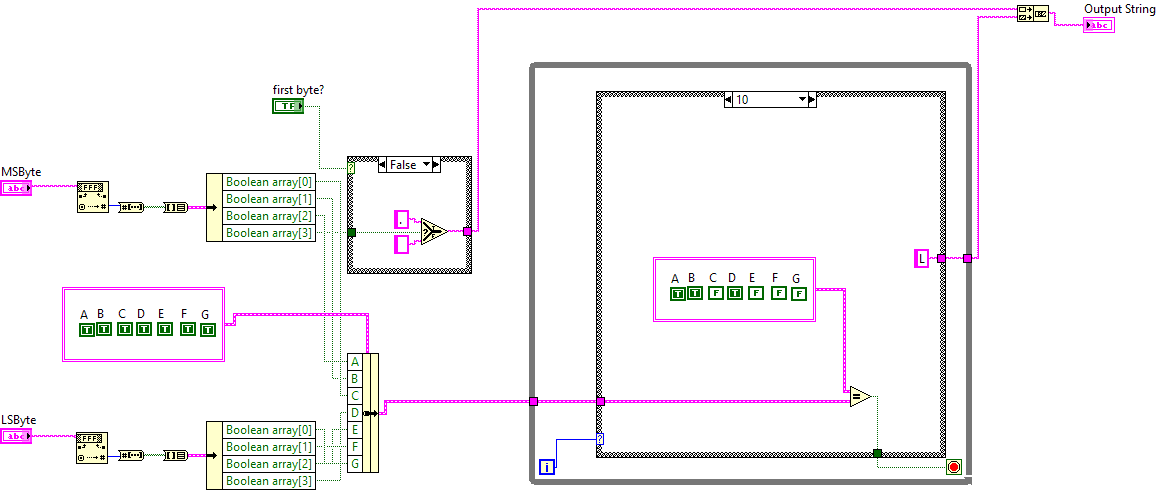
\includegraphics[width=1\linewidth]{lv/dmm/DMM_lvclass_bitcoded}
                \caption{Captura de tela do transformação de 7bitcode em string de números}
                \label{fig:dmmbitcode}
            \end{figure}
            
            
            \begin{figure}
                \centering
                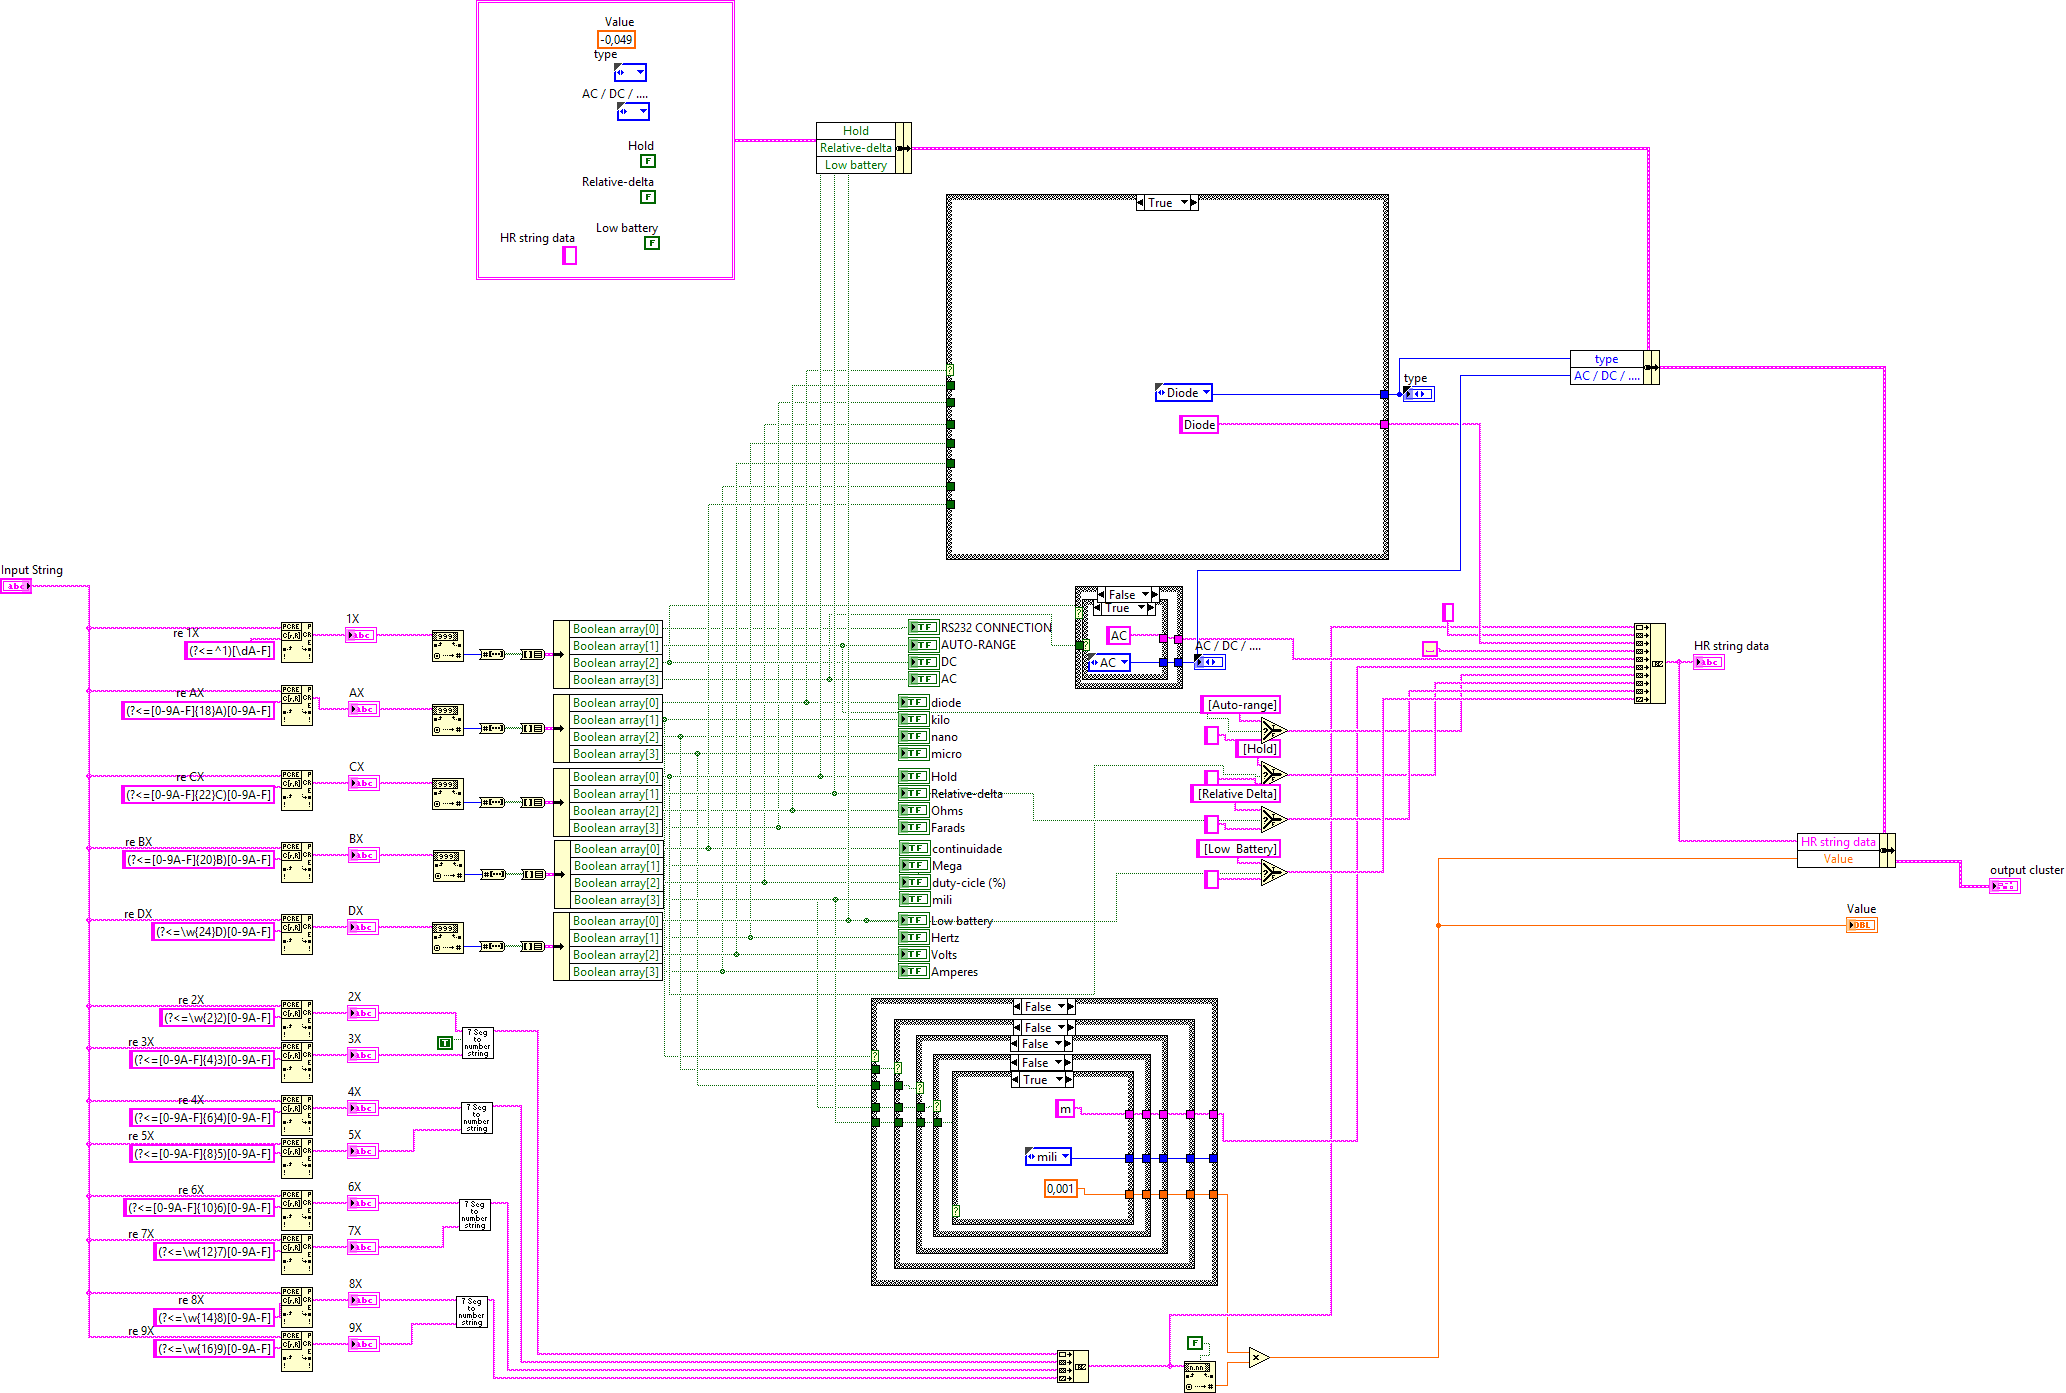
\includegraphics[width=1\linewidth]{lv/dmm/DMM_lvclass_DMM_RS232_14bit_parserd}
                \caption{Captura de tela do Parser da serial}
                \label{fig:dmmparser}
            \end{figure}
            
            
            \begin{figure}
                \centering
                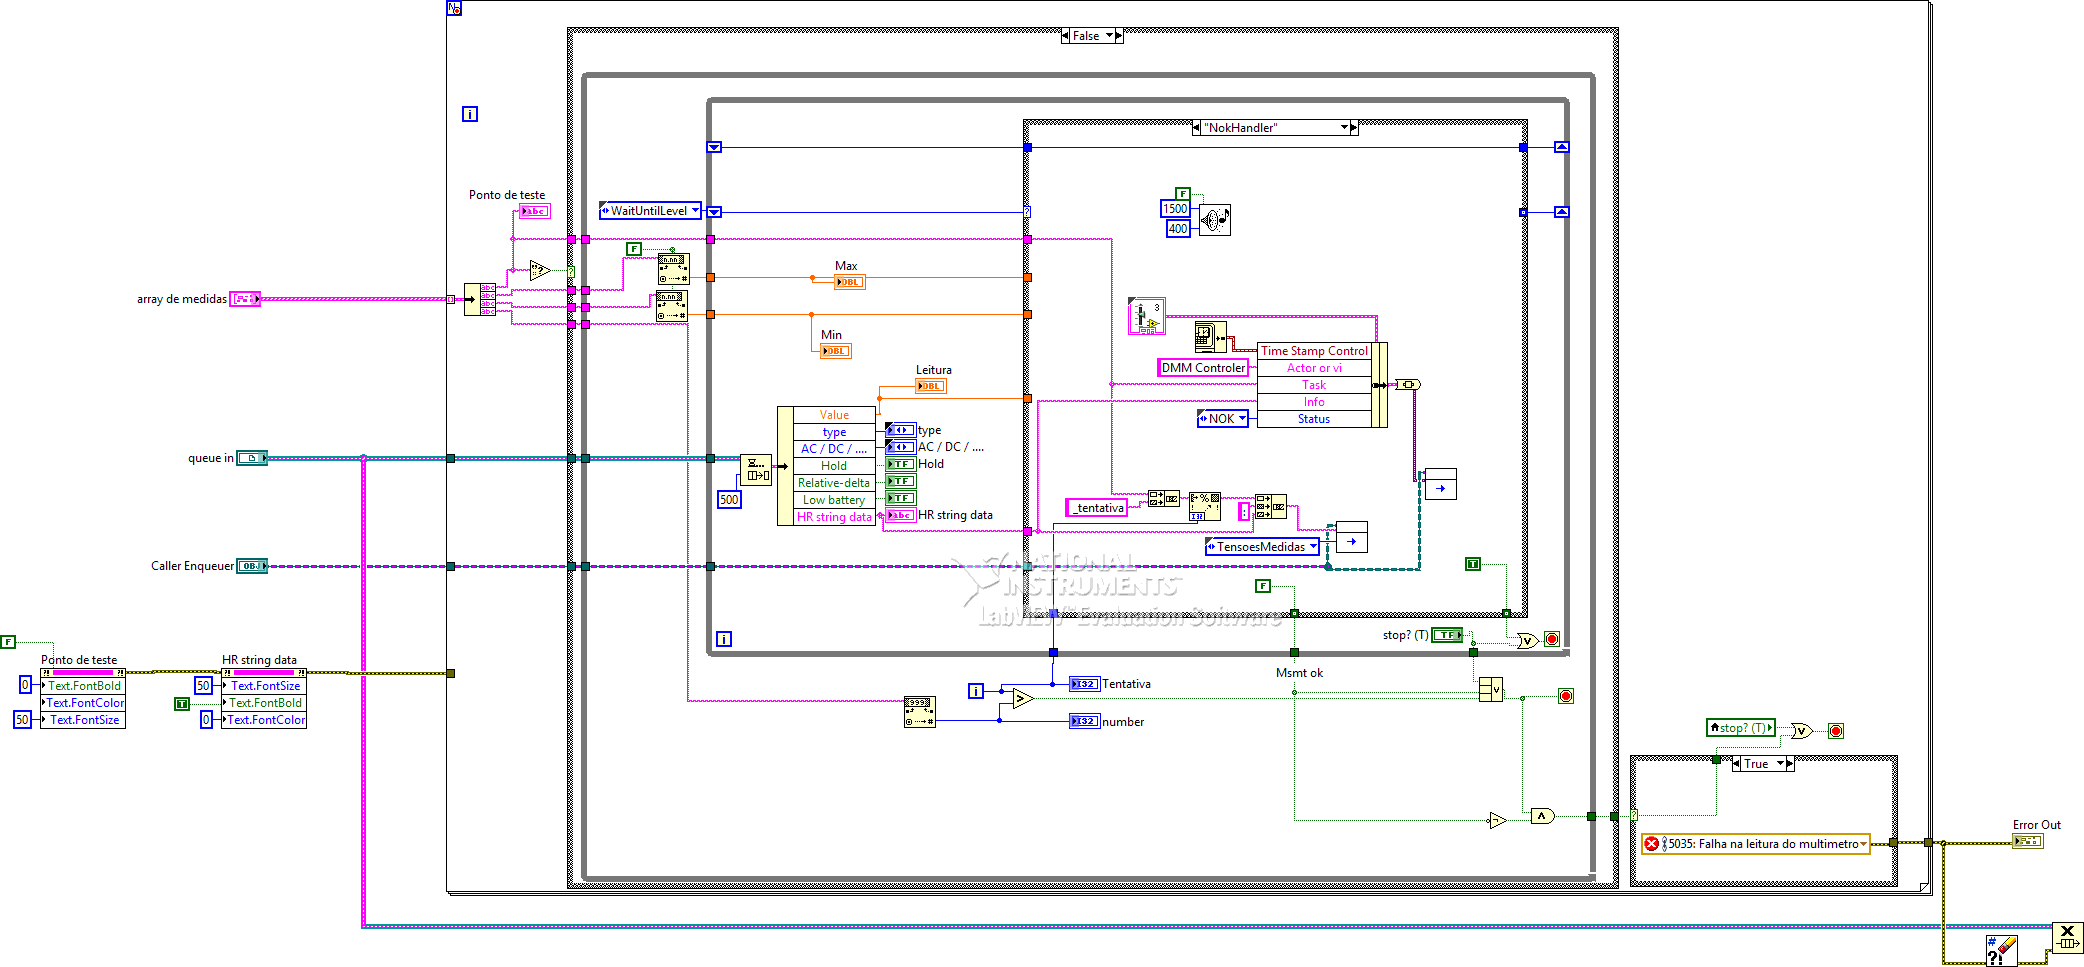
\includegraphics[width=1\linewidth]{lv/dmm/DMM_lvclass_DMM_UI_d}
                \caption{Captura de tela do Diagrama de blocos da interface de usuário}
                \label{fig:dmmfpbd}
            \end{figure}
            
            \begin{figure}
                \centering
                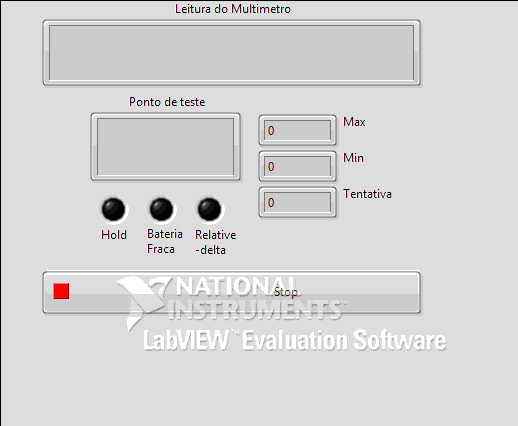
\includegraphics[width=1\linewidth]{lv/dmm/DMM_lvclass_DMM_UI_p}
                \caption{Captura de tela do Painel frontal da interface de usuário}
                \label{fig:dmmfp}
            \end{figure}
            
            
        \clearpage
        \subsection{Implentação do gerador de registros}
            
            O gerenciador de registros neste programa basicamente recebe todos os dados da execução das baterias de teste e aglutina em um documento, possibilitando a geração de arquivos de texto como também a de arquivos JSON.
            
            Mesmo que o ator suporte o envio dos arquivos para um servidor, o armazenamento dos arquivos é feito em pastas locais, já que o \textit{webservice} de registros ainda não foi adaptado para este programa.
            
            A saída padrão deste ator é composta por duas classes de registros: 
            
            Um registro com todos os dados de execução, despejo dos dados da serial, \textit{timestamps}, e com os registros de exceções de execução. Dados necessários para a depuração de problemas na placa, e para melhor efetividade no retrabalho.
            O segundo registro consiste em um resumo da bateria de testes, diagnóstico geral da placa, e qualquer informação que for valiosa para análise em massa, requisito necessário para otimizações do processo produtivo como também do próprio produto.
            
            Nas figuras \ref{fig:loggen} e \ref{fig:logmake} vemos os diagramas de blocos dos instrumentos virtuais internos desta classe, responsáveis para criação dos arquivos de registro de execução.
            
            \begin{comment}
                \begin{figure}
                    \centering
                    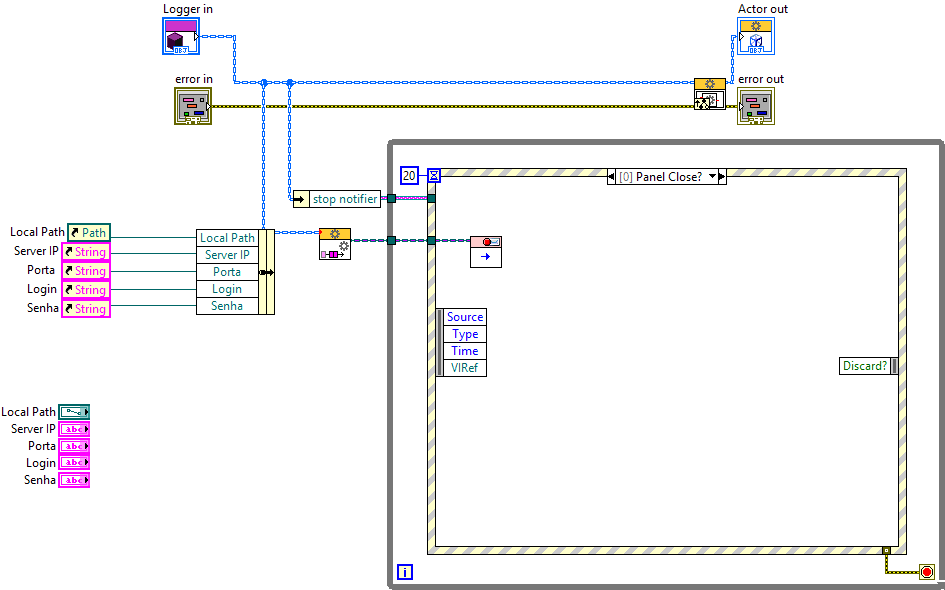
\includegraphics[width=1\linewidth]{lv/log/Logger_lvclass_Actor_Cored}
                    \caption{Captura de tela do Actor Core do Gerador de Log}
                    \label{fig:logcore}
                \end{figure}
                \begin{figure}
                    \centering
                    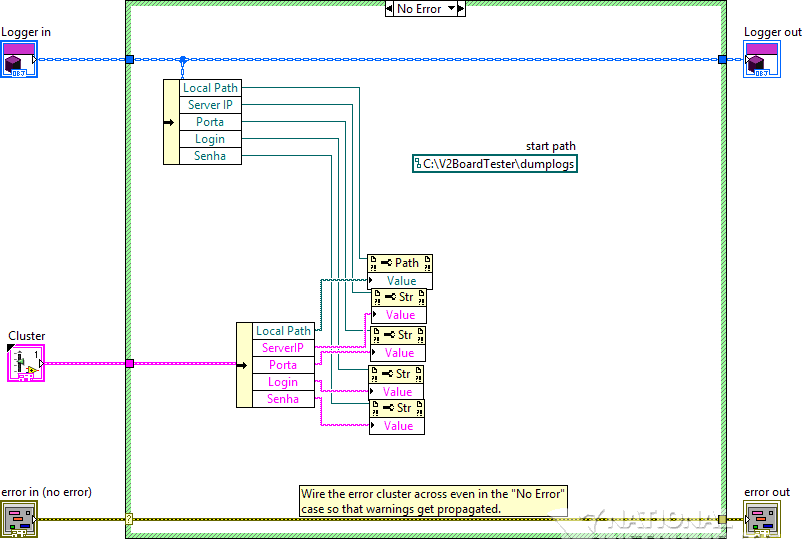
\includegraphics[width=1\linewidth]{lv/log/Logger_lvclass_Configd}
                    \caption{Captura de tela do Configurador Gerador de Log}
                    \label{fig:logconf}
                \end{figure}
            \end{comment}
            
            
            \begin{figure}
                \centering
                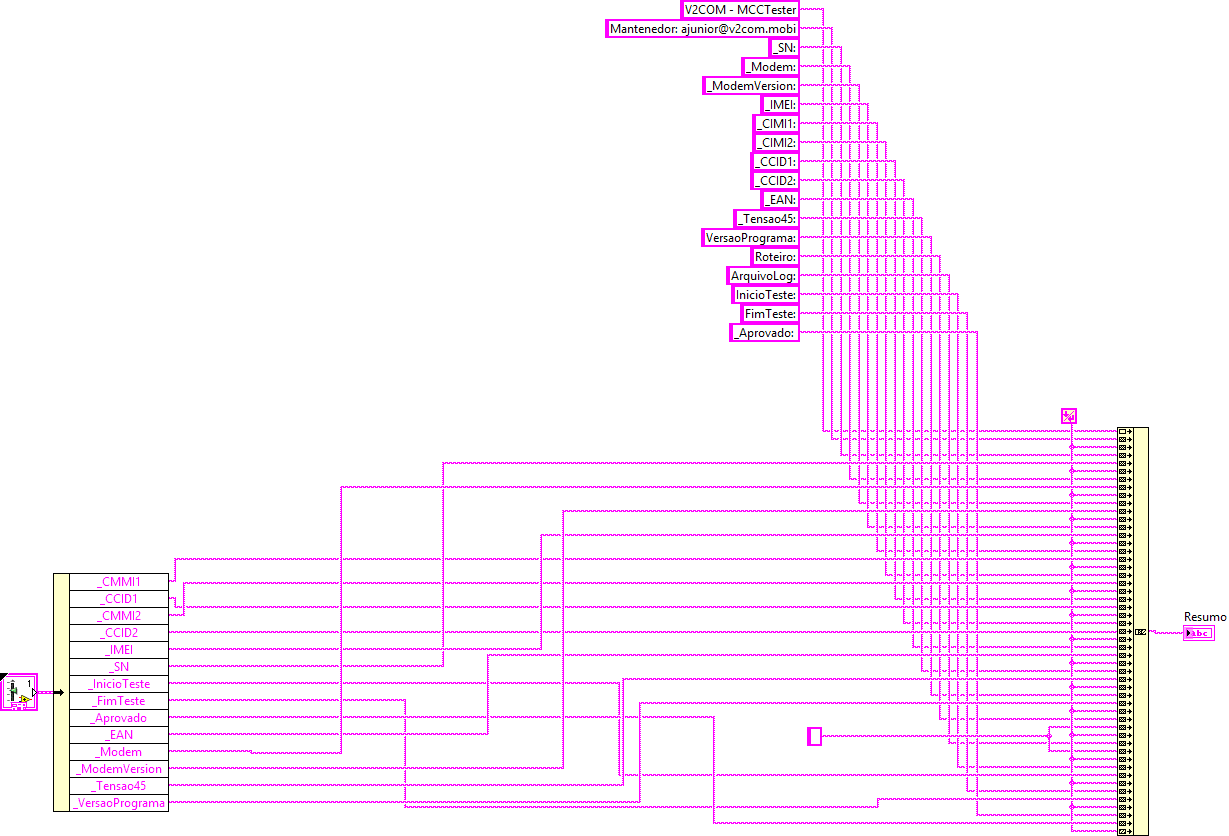
\includegraphics[width=1\linewidth]{lv/log/Logger_lvclass_LogGen_(SubVI)d}
                \caption{Captura de tela do Instrumento virtual de geraçao de log}
                \label{fig:loggen}
            \end{figure}
            \begin{figure}
                \centering
                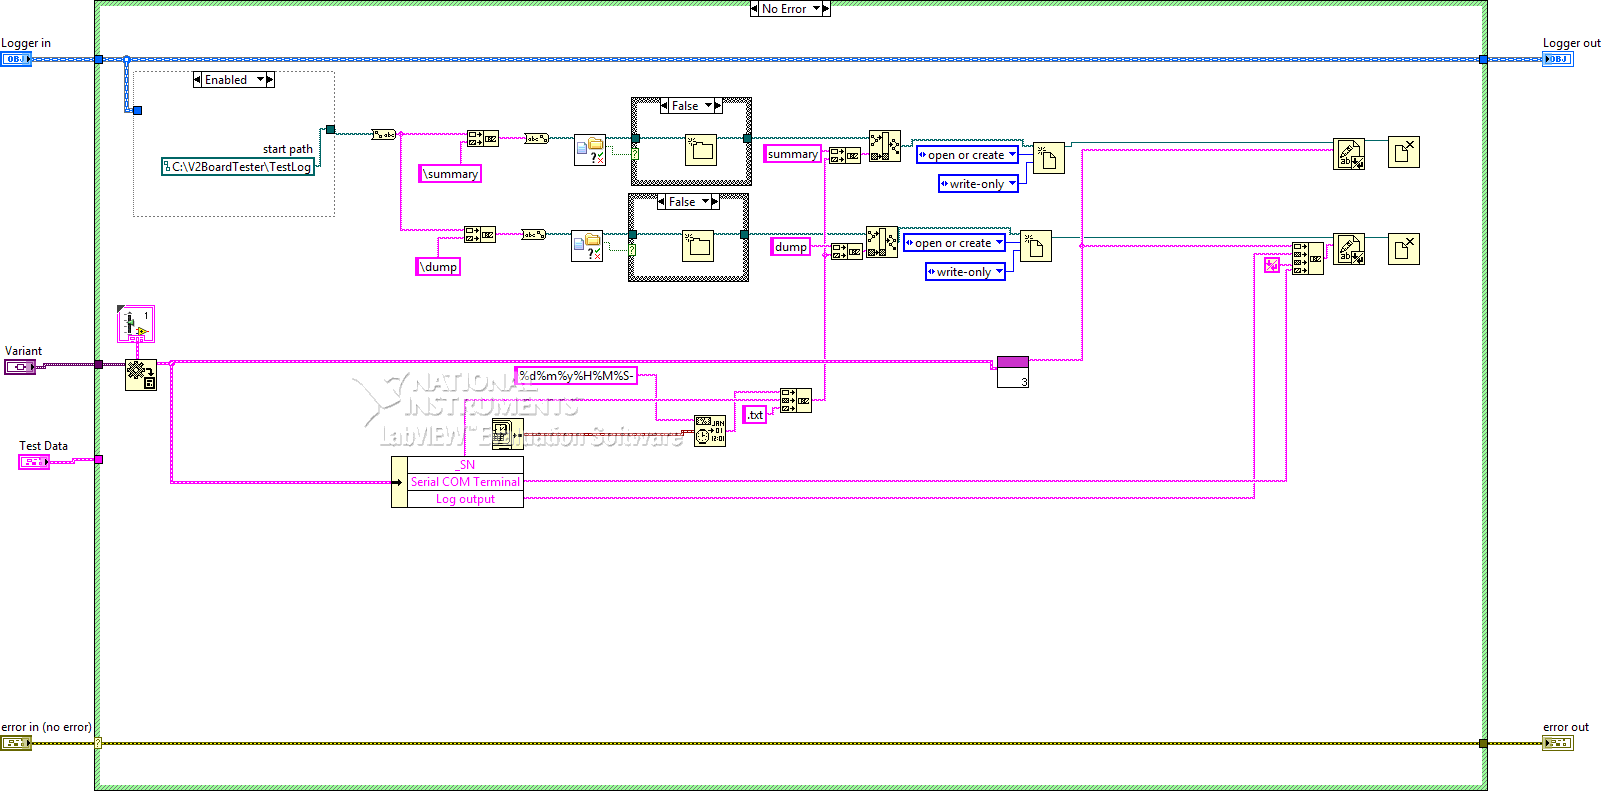
\includegraphics[width=1\linewidth]{lv/log/Logger_lvclass_MakeLogd}
                \caption{Captura de tela do Criador  de Log}
                \label{fig:logmake}
            \end{figure}
            \clearpage   
        \subsection{Implentação do medidor de potência}
            
            Como explicado na sessão \ref{pwmodel}, a implementação do medidor de potência de sinal do \textit{front-end} foi feita parcialmente, já que é realizada por outro programa e em outra etapa do processo produtivo.
            
            Apesar de fora deste escopo de trabalho, ressalta-se que foram realizados melhorias e otimizações no processo de medição de potência de front-end também.
            
            As figuras \ref{fig:pwcore} e \ref{fig:pwconf} exibem o diagrama de blocos dos instrumentos virtuais do Actor Core e de configuração do ator, respectivamente. A implementação de outros módulos dependem do interesse da empresa de realizar este teste nas empresas que prestam os serviços de montagem.
            
            \begin{figure}
                \centering
                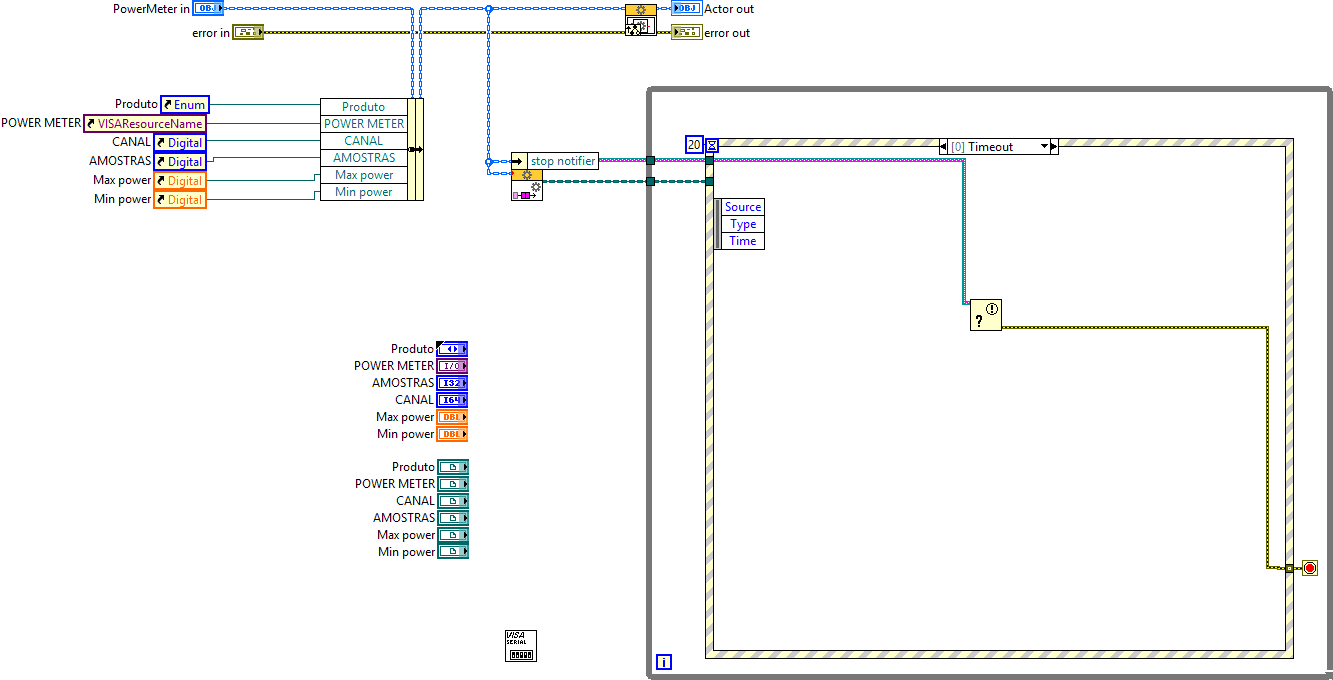
\includegraphics[width=1\linewidth]{lv/pwmtr/PowerMeter_lvclass_Actor_Cored}
                \caption{Captura de tela do Actor Core do Power Meter}
                \label{fig:pwcore}
            \end{figure}
            \begin{figure}
                \centering
                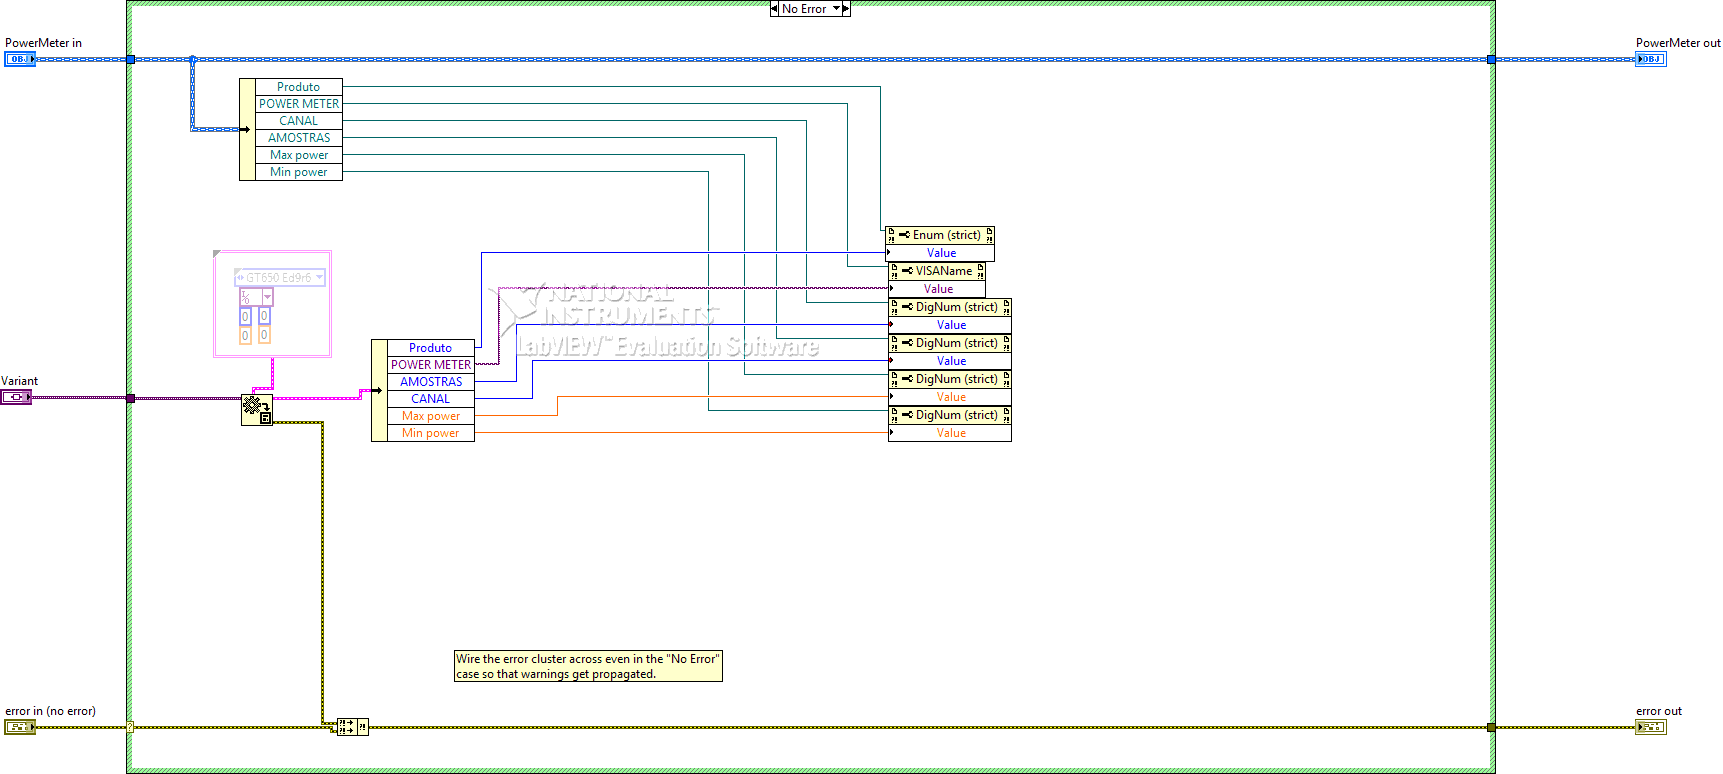
\includegraphics[width=1\linewidth]{lv/pwmtr/PowerMeter_lvclass_SET_PM_Actor_Configd}
                \caption{Captura de tela do Configuração do Power Meter}
                \label{fig:pwconf}
            \end{figure}
        \clearpage
        \subsection{Implentação do controlador}
        
        O actor core, como qualquer outro módulo do programa (figura \ref{fig:cntrlcore}). Por centralizar e fazer o controle de fluxo de teste, através de mensagens de execução e respostas sobre o status de execução, o controlador foi implementado com uma estrutura orientada à eventos. Dessa maneira, sempre que ele receber resposta de um ator filho, ele pode disparar outras mensagens de execução.
        
        Conforme já mencionado, um ator só entende mensagens que invocam métodos internos dele. Com isso em mente, foi criado um método especifico para relatar sucesso/falha de execução de subrotinas dos atores filhos ao controlador. Esta mensagem, enviada pelos atores-filhos, invoca o método interno do controlador, \textit{report control flag.vi} (figura \ref{fig:cntrlset}), o qual dispara outros eventos mencionados no parágrafo anterior.
        
        \begin{figure}
                \centering
                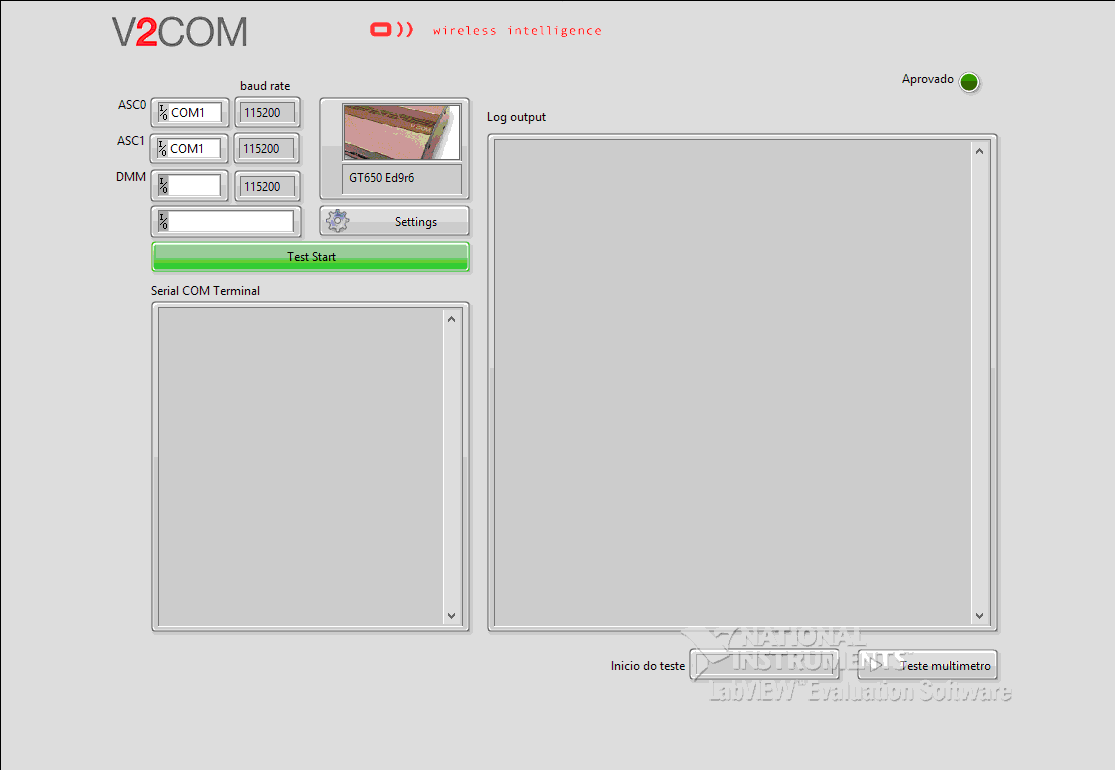
\includegraphics[width=0.8\linewidth]{lv/controler/Controller_lvclass_Actor_Corep}
                \caption{Captura de tela do Painel Frontal para a interface de usuário}
                \label{fig:cntrlpanel}
        \end{figure}
        
        \begin{figure}
                \centering
                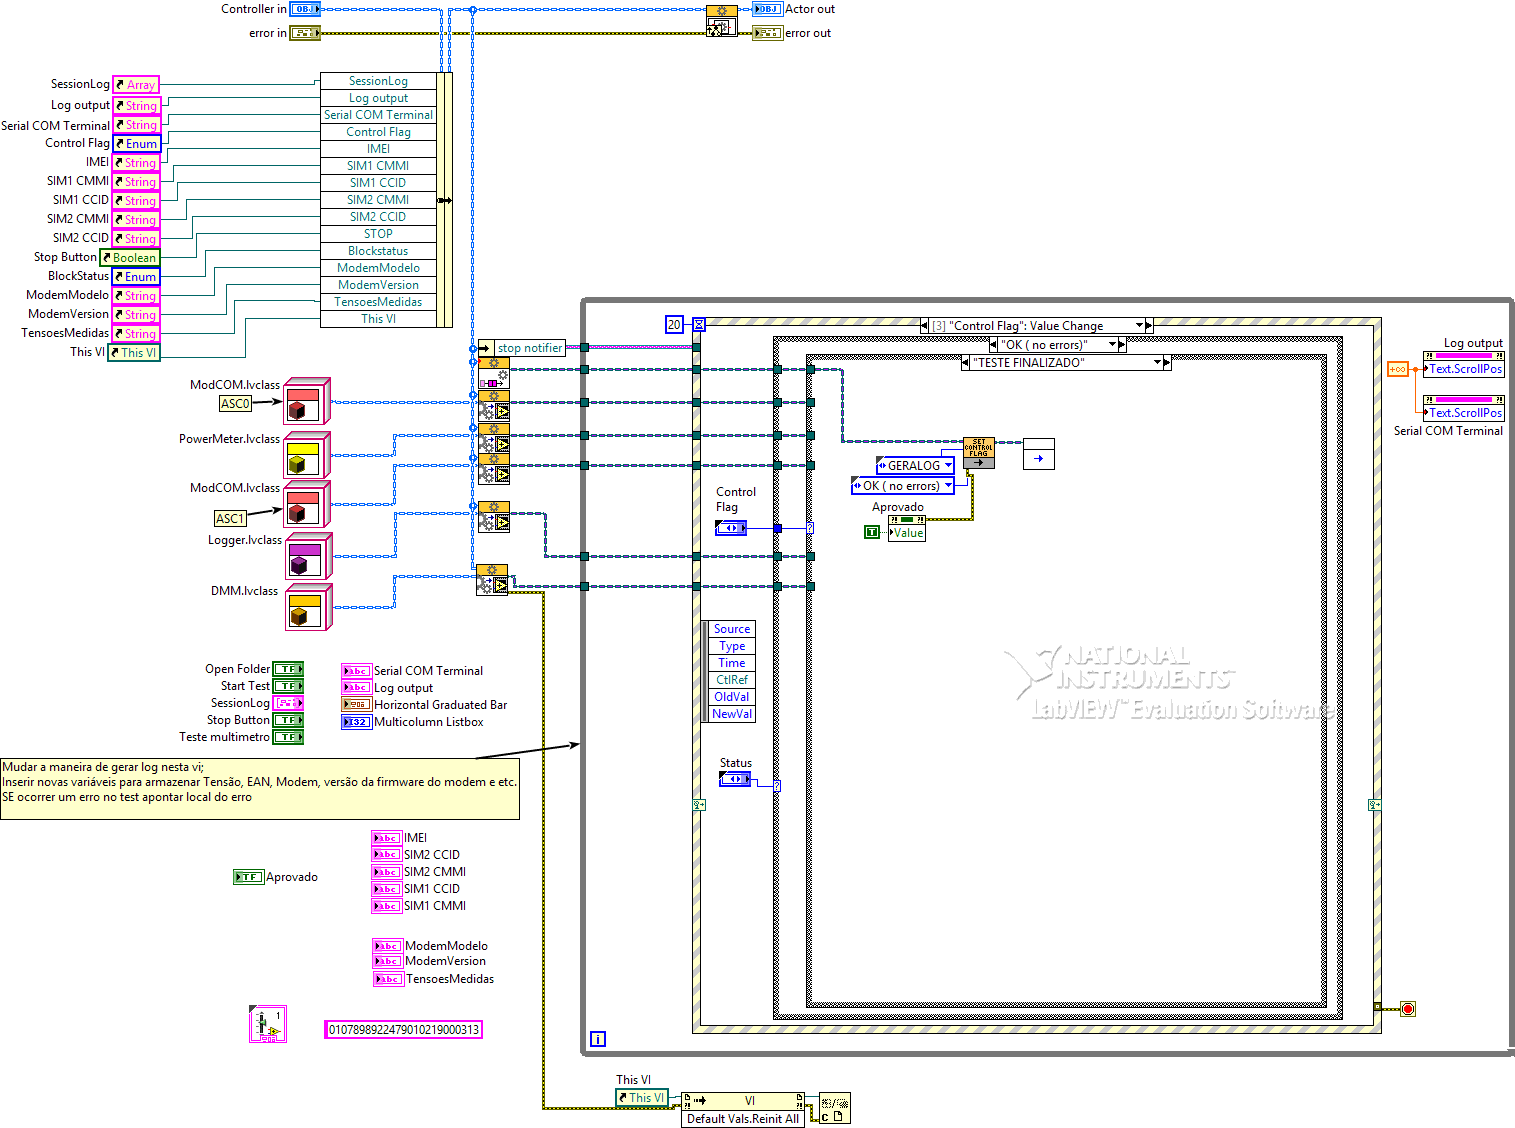
\includegraphics[width=1\linewidth]{lv/controler/Controller_lvclass_Actor_Cored}
                \caption{Diagrama de blocos do \textit{Actor Core.vi} do Controlador}
                \label{fig:cntrlcore}
        \end{figure}
        
        Vemos também na figura \ref{fig:cntrlcore}, que este ator inicializa todos os outros atores filhos logo no inicio de sua execução. Seu inicializador pode ser visto na figura \ref{fig:cntrlprestop}.
        
        Da mesma forma que os atores filhos se comunicam com o controlador pelas mensagens sob sua competência, este só pode enviar mensagens que aqueles possam entender.
        
        \begin{figure}
                \centering
                \begin{subfigure}[b]{0.45\textwidth}
                    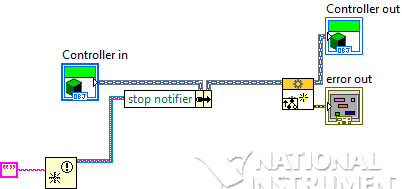
\includegraphics[width=1\linewidth]{lv/controler/Controller_lvclass_Pre_Launch_Initd}
                    \caption{VI de pré-inicialização}
                \end{subfigure}
                \begin{subfigure}[b]{0.45\textwidth}
                    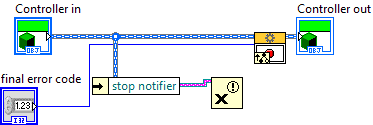
\includegraphics[width=\linewidth]{lv/controler/Controller_lvclass_Stop_Cored}
                    \caption{VI de parada}
                \end{subfigure}
                \caption{Capturas de tela das VI de pré-inicialização e parada do Ator}
                \label{fig:cntrlprestop}
        \end{figure}
        
        \begin{figure}
                \centering
                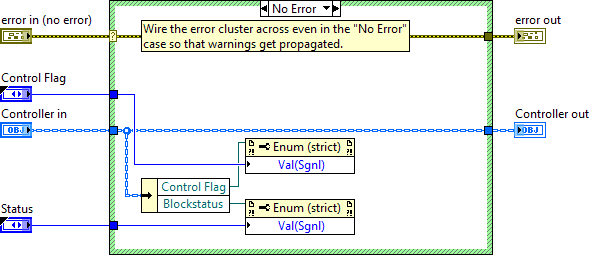
\includegraphics[width=0.9\linewidth]{lv/controler/Controller_lvclass_SET_Control_Flagd}
                \caption{Captura de tela do método interno que recebe a mensagem do bloco de teste executado e seu status de conclusão.}
                \label{fig:cntrlset}
        \end{figure}
        
    
        \clearpage
    \clearpage
    \chapter{Análise de execução}
    
        Com o programa pronto, foi montado um esquema de teste internamente, sem que fosse à fábrica, para avaliá-lo em relação à versão anterior em Java. Foram separadas cerca de 20 placas e testadas com ambos os programas.
        
        Após isso, foram mensurados os tempos de execução de teste. A figura \ref{tab:resultado} exibe as médias dos resultados para os dois programas. Nota-se pela imagem, uma redução de quase 10 segundos no tempo médio de teste. Observa-se que estes resultados são atribuídos somente pelas mudanças ergonômicas do programa, já que o roteiro é idêntico ao anterior. Questões de velocidade de processamento entre as linguagens não refletiram em muitas mudanças, se considerarmos que nenhuma das atividades exigem uso intenso de CPU, e que o gargalo do teste é interno ao modem. Certamente que resultados melhores podem ser obtidos se aproveitados os recursos de concorrência de \textit{software} que \textit{framework} oferece. Isso foge do escopo deste trabalho, que se propôs somente em oferecer uma base para o teste concorrente de placas eletrônicas.
        
    \begin{table}[]
        \centering
        \caption{Média e desvio padrão das 20 amostras de teste de bancada}
        \label{tab:resultado}
        \begin{tabular}{l|cc}
        
                          & Programa Legado & Modelo de Atores \\
    \hline
            Média (seg)         & $33.65\pm2.43$          & $26.24\pm3.37$                          \\
        \end{tabular}
        \end{table}
        
    \begin{comment}
        Com o programa pronto, foi montado um esquema de teste para avaliá-lo em relação à versão anterior em Java. 
        Foi separado um lote de 200 placas e testadas metade com o primeiro programa, e outra metade com o outro.
        
        A partir destes estados, foram levantados os tempos de execução de cada teste que são exibidos na figura \ref{fig:resultado}. Observa-se pela imagem, uma redução considerável no tempo mínimo e médio de teste. Passando de 
        
        Observa-se que estes resultados foram obtidos somente com a mudança de uma linguagem interpretada para uma compilada, e melhor elaboração do programa, Já que o roteiro é idêntico ao anterior. Certamente que resultados melhores podem ser obtidos se aproveitados os recursos de concorrência de \textit{software} que \textit{framework} oferece. 
        
        Nota-se também que a distribuição dos tempos de teste do programa novo é ligeiramente mais difusas do que o do programa antigo, que pode ser atribuído à falta de hábito dos operários com a nova interface.
        
        Também foram observados a quantidade de erros existentes no programa durante as etapas que envolvem interação com o operador. Esses erros analisados estão aqui representados na figura \ref{fig:erros}. Como esperado, melhorias ergonômicas reduziram o tempo de teste, e taxa de erro de operador.
        
        
        \begin{figure}
            \centering
            \includegraphics{}
            \caption{taxa de erro nas baterias de teste que envolvem o operador}
            \label{fig:erros}
        \end{figure}
\end{comment}        

   \section{Conclusão}
       
        
        Neste trabalho, não foi realizada nenhuma análise crítica do roteiro de testes e sua efetividade de cobertura. Isso se torna imprescindível, considerando os dados internos da manutenção que frequentemente reportam \textit{"causa desconhecida"} sobre os retornos de campo.
        
        O uso da linguagem gráfica do ambiente \textit{Labview} apesar de simples para pequenas rotinas, torna-se complicado e difícil de refatorar ao aplicado a programas maiores, e sua implementação do paradigma orientado à objetos assim como do modelo de atores é demasiadamente complicada e problemática de usar.
        Uma maneira de contornar isto seria, talvez a utilização do Labwindows\texttrademark/CVI, o ambiente C da National Instruments, ou o uso do Labview somente em partes aonde ele se sobressalta como melhor opção.
        
        O principal problema encontrado foi o escrever o roteiro da bateria de testes no código fonte do programa. Isso inflexibiliza a equipe em relação à mudanças
        
        Dentre as melhorias interessantes para o processos de teste de placas, destacam-se:
        \begin{itemize}
            \item Paralelização do roteiro e melhor uso dos recursos da concorrência de software.
            \item Roteiro como arquivo de entrada do programa, interpretado por um módulo interno do programa.
            \item Envio automático e criptografado do roteiro ao sistema de registros de teste da fábrica. Atualmente isso é realizado manualmente.
            \item Teste de potência RF serem realizados em conjunto com os testes em fábrica.
            \item Construção de uma giga de testes que suporte múltiplas placas sendo testadas simultaneamente. No aspecto de software, isso demandaria o desenvolvimento de um ator numa camada superior ao controlador - tarefa sem grandes dificuldades.
        \end{itemize}
        
        Feitas as críticas, ressalta-se que o modelo de atores se mostrou apropriado para modelar vários módulos de software concorrentes, e escalona bem para aplicações maiores. 
        